% New translation authored from the final approved Chinese manuscript.
% The previous English manuscript is NOT used as prose source.
% Springer Nature sn-jnl / Cybersecurity double-anonymous manuscript.
\documentclass[referee,lineno,pdflatex,sn-basic,Numbered]{sn-jnl}
\usepackage{amsmath,amssymb,amsthm,booktabs,graphicx,tabularx}
\usepackage{url}
\emergencystretch=2em
\newtheorem{proposition}{Proposition}
\newtheorem{lemma}{Lemma}
\begin{document}
\title[Robust spacetime certification]{Zero-Knowledge Certification of Robust Spacetime Compliance under Byzantine Evidence for Vehicular Crowdsensing}
\author[1]{\fnm{Anonymous} \sur{Authors}}
\affil[1]{\orgname{Withheld for double-anonymous review}}
\abstract{In vehicular crowdsensing, a location-privacy mechanism may need to establish compliance with a spatial policy without revealing a vehicle's coordinates. Yet positioning errors, environmental effects, and synchronization uncertainty often leave only interval-valued spacetime observations. Even authenticated sources may share systematic bias or behave in a Byzantine manner. We propose a privacy-preserving compliance certification method based on signed spacetime uncertainty evidence. Given an upper bound $f$ on Byzantine issuers and an allowance $r$ for honest issuers whose intervals miss the true event, the method constructs the feasible set of states supported by at least $k=n-f-r$ issuers. A report is accepted only when this set is nonempty and wholly contained in the authorized region. The resulting decision distinguishes valid, invalid, ambiguous, and inconsistent evidence. We implement two Groth16/BN254 circuits that verify EdDSA/MiMC signatures and bind the proof to the task, issuer roster, report, threshold, challenge nonce, and expiry. Gateway tests reject tampering, context substitution, expired challenges, and cross-challenge replay; only one of eight concurrent copies of a valid request is accepted within a single gateway instance. Across 12 synthetic conditions satisfying the configured fault and coverage assumptions, mean decisive coverage is 87.52\%, compared with 75.63\% for a fixed-margin baseline. Tested subset circuits produce 164-byte proofs with median proving times of 163--255 ms on an Apple M1. The implementation is an evidence-certification layer, not a complete vehicular crowdsensing platform; its physical interpretation still depends on trusted issuer enrollment and effective sensor calibration.}
\keywords{Zero-knowledge proofs, Location privacy, Vehicular crowdsensing, Byzantine evidence, Robust evidence fusion, Spacetime compliance certification}
\maketitle
\section{Introduction}
In location-privacy applications, a verifier may need to establish that a user satisfies a spatial policy without learning the user's precise coordinates. Zero-knowledge location proofs, for example, can verify membership in a designated region while keeping the location private~\cite{ZKLP,VehiclePolicy}. Such verification commonly starts from a definite spacetime position. Vehicle sensing, however, cannot always provide an observation of that kind. Positioning error, environmental interference, and clock-synchronization uncertainty may restrict the available evidence to a range of plausible positions and times. A valid source signature authenticates the evidence submitted by that source; it does not establish that the physical estimate is accurate. Compromised sources may also sign deliberately misleading observations. Consequently, even a mathematically correct proof concerning a hidden coordinate does not establish that the chosen coordinate is sufficiently supported by observations. This paper asks how multiple uncertain, and potentially malicious, spacetime observations can support a policy-compliance claim without being disclosed to the verifier.

The problem is particularly relevant to vehicular crowdsensing. Distributed vehicle observations support traffic monitoring, road management, and environmental-sensing tasks~\cite{Suhag2023,Zheng2025BARM}, for which the admissibility of a report may depend on the event's location and time. Revealing the positioning evidence can expose a vehicle's mobility history. Replacing several interval-valued observations with one representative point, however, can conceal disagreement near a policy boundary. Requiring every source interval to intersect is not necessarily safer: a Byzantine issuer may submit a displaced interval that excludes the true state while leaving a small intersection entirely within the authorized region. A sound compliance rule therefore needs to specify which possible states have sufficient evidential support and how conflicting observations are handled, in addition to protecting those observations.

We consider privacy-preserving compliance certification over signed spacetime uncertainty evidence. Each enrolled issuer signs an axis-aligned integer box for the same reference event. For $n$ issuers, at most $f$ Byzantine sources, and at most $r$ honest observations that fail to cover the true state, let $k=n-f-r$. The robust feasible set $\mathcal F_k$ consists of the states covered by at least $k$ signed boxes. Compliance is certified only if this set is nonempty and entirely contained in the authorized policy. A nonempty feasible set lying outside the policy produces an invalid decision; a set crossing the boundary is ambiguous; and a set with no threshold-supported state is inconsistent. A valid decision is reserved for the acceptance condition. These four outcomes avoid treating an arbitrarily chosen point as conclusive and distinguish a conflict in otherwise valid evidence from failure to submit the required evidence.

We combine threshold-based fault-tolerant interval reasoning~\cite{Marzullo1990,BFTPoLoc,PG,CRSF} with zero-knowledge certification. Rather than revealing the source intervals, the prover establishes that the signatures satisfy the roster and context constraints and that the reported decision follows from the same threshold rule. A report-binding protocol associates this proof with the task, issuer roster, report bytes, threshold, challenge nonce, and expiry. This association prevents a proof for one authorized context from being reused as evidence for another, under the stated cryptographic and gateway assumptions.

The scope is an evidence-certification module that can be integrated into a vehicular crowdsensing application, not a platform that also performs participant recruitment, incentives, or dynamic issuer governance. Signatures and zero-knowledge proofs can enforce source authentication, contextual binding, and the specified computation; inference about the physical event additionally requires trustworthy enrollment, adequate calibration, and coverage by enough honest sources. We keep these physical premises separate from cryptographic guarantees throughout the security analysis.

The contributions are summarized as follows:
\begin{itemize}
\item \textbf{Four-valued certification under explicit fault and coverage budgets.} We use the set of threshold-supported spacetime states as the object of policy verification, distinguish valid, invalid, ambiguous, and inconsistent evidence, and establish conditional soundness when the true state is covered by sufficiently many honest sources.
\item \textbf{Two exact finite-domain proof circuits.} Lower-corner maximum-depth reachability and threshold-subset enumeration establish the same four-valued relation. Both are instantiated with Groth16/BN254, verify EdDSA/MiMC signatures within the circuit, and constrain the private evidence to the public policy, roster, threshold, and report context.
\item \textbf{A task-bound verification gateway.} The gateway reconstructs public inputs from a trusted task configuration, checks roster consistency, verifies the proof, and atomically marks a successfully used challenge as consumed. Protocol tests examine evidence tampering, task/report substitution, expired challenges, and concurrent replay within one gateway instance.
\item \textbf{Semantic and cryptographic evaluation.} We examine 64,800 synthetic observations, paired re-evaluations under different honest-miscoverage allowances, replay on 787 measured UrbanNav reference states with simulated multisource evidence, 300 measured Groth16 proof executions across two circuit backends, and resource-limited circuit compilation. A fixed-version reproduction of an open-source location-proof baseline provides additional implementation context. None of these experiments is presented as an in-field calibration trial of real multisource vehicular sensors.
\end{itemize}

Figure~\ref{fig:architecture} depicts the certificate workflow. Issuers authenticate uncertainty regions associated with the same report; the vehicle uses the regions and signatures as a private witness; and the gateway checks the public task context and accepts the report only after verifying a valid classification. The witness is hidden from the verifier, but the report content, public policy, and classification can remain visible.

\begin{figure}[htbp]\centering
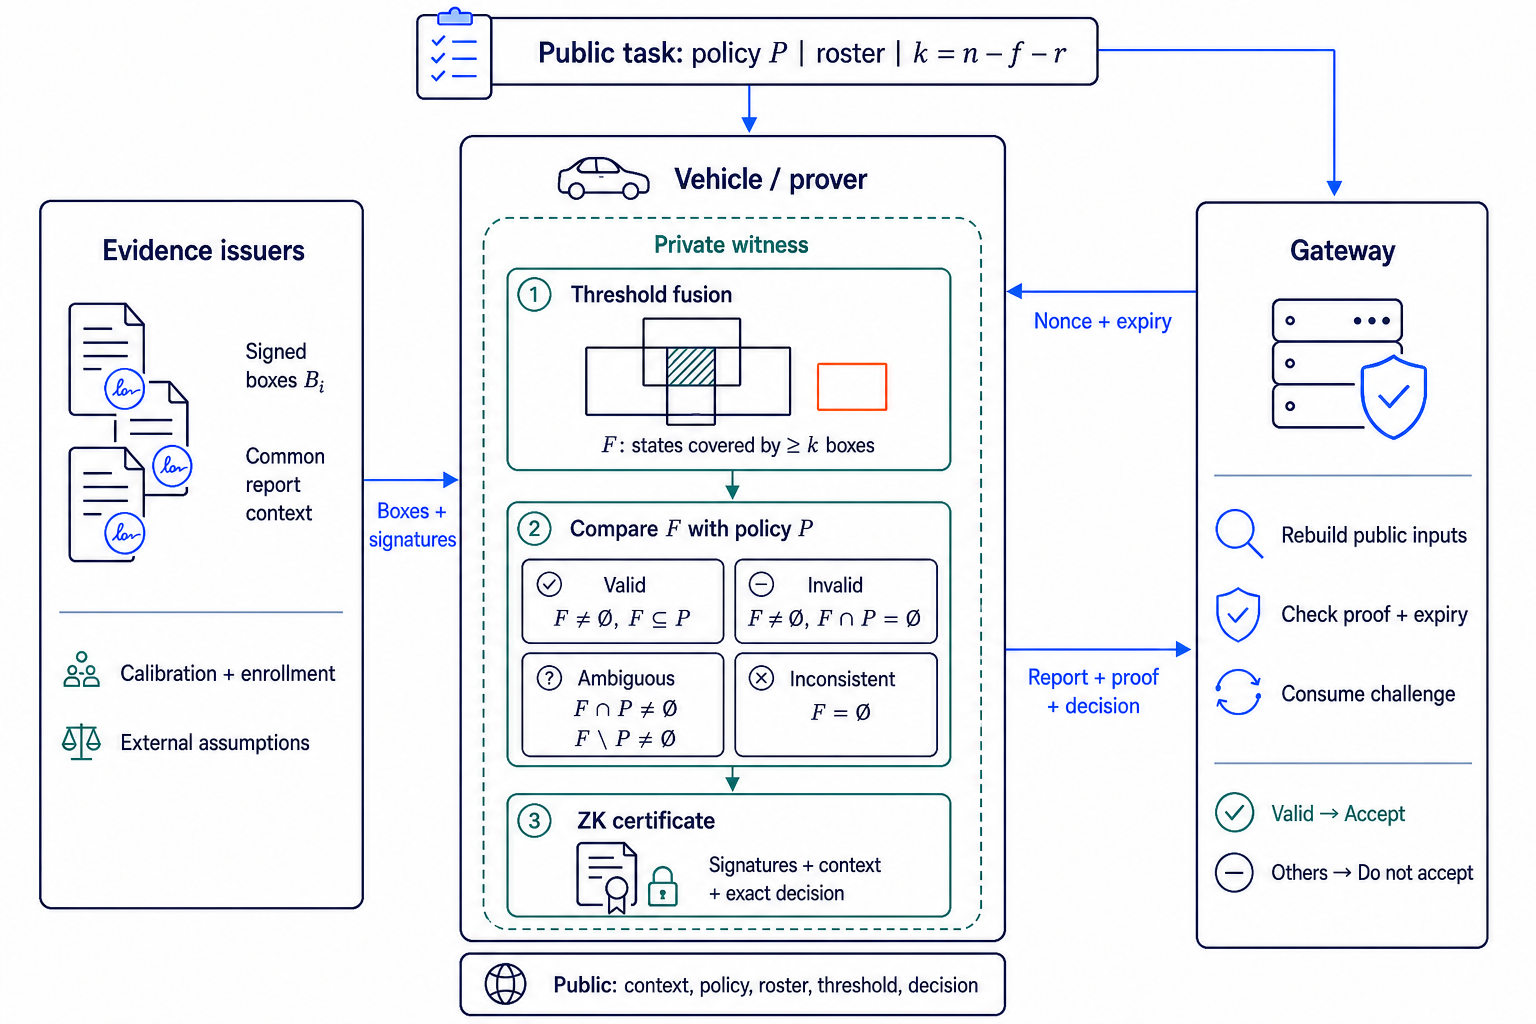
\includegraphics[width=\linewidth]{../figures/system_architecture.png}
\caption{Conceptual architecture of the evidence-certification module. Labels $B_i$ and $F$ in the diagram correspond to signed boxes $U_i$ and the feasible set $\mathcal F_k$. An inconsistent decision is a semantic outcome for complete, authenticated evidence; missing or malformed evidence instead aborts the protocol. Coordinates are task-defined integers obtained through conservative quantization. Sensor calibration, trusted enrollment, and institutional independence are external assumptions, not properties established by the diagram or proof circuit.}\label{fig:architecture}
\end{figure}

Section~2 reviews relevant work on vehicular privacy, zero-knowledge location verification, and Byzantine-robust fusion. Section~3 develops the model and circuits; Section~4 establishes their security boundary; Section~5 presents the experiments; and Section~6 concludes.

\section{Related Work}
\subsection{Privacy and trustworthy crowdsensing in vehicular networks}
Research on vehicular crowdsensing security has addressed participant identity, confidentiality of sensed data, and evidence trustworthiness. AARE combines anonymous authentication with privacy-preserving assessment of data reliability~\cite{Cheng2023}. BARM introduces blockchain-assisted anonymous authentication and reputation management to evaluate and update participant reputations~\cite{Zheng2025BARM}. Regarding data processing, PPVDA studies privacy-preserving and verifiable aggregation~\cite{Zhou2024}; BCS-LPP employs techniques including Geohash and order-preserving encryption to protect sensing locations while supporting location checks and task management~\cite{Shen2024}. Cooperative detection of anomalous vehicular behavior has also been investigated at both vehicle and roadside-unit levels~\cite{Sultana2024}. Other recent work examines lightweight anonymous authentication, certificateless aggregate signatures, and SNARK-based verification of computations on authenticated data~\cite{Imam2025JISA,Wang2025JISA,Reinhart2026ADSC}. Recent work in \emph{Cybersecurity} extends this authentication perspective in different settings: Umrani and Palmieri investigate threshold password-authenticated key exchange for vehicular ad hoc networks~\cite{CybersecUmrani2025}, while Wang et al. develop privacy-preserving multi-authority aggregate signatures for smart-grid message authentication~\cite{CybersecWang2026}. These systems address secure communication or message authentication, rather than the physical coverage of uncertain evidence.

These approaches strengthen privacy and trust at different points in the sensing workflow, but they certify different objects. Identity authentication establishes participation rights; private aggregation protects inputs and checks computation; and misbehavior detection identifies suspicious participants. In the setting addressed here, several authenticated sources provide uncertain or conflicting spacetime observations about one event. Source legitimacy and signature validity alone do not establish whether the event complies with a given policy. The additional requirement is a verifiable basis for a policy decision that retains the uncertainty of the individual observations.

\subsection{Zero-knowledge location and geometric-policy verification}
Location privacy can be pursued through application-specific obfuscation and protected queries~\cite{Mdee2022,Atmaca2024}, or by credentials and authentication protocols that limit the disclosure of sensitive location information~\cite{Ghani2025,Zhang2025Sybil,Wang2025ZKAuth}. Zero-knowledge proofs offer another approach: a verifier can check a geometric constraint without learning the protected coordinate or an entire trajectory. ZKLP, proposed by Ernstberger and colleagues, incorporates floating-point geometry into zero-knowledge proofs for region membership and proximity predicates~\cite{ZKLP}. The vehicle-policy protocols of Bogdanov and colleagues instead use locations signed by a trusted witness to prove compliance with driving-area requirements in subsidy or taxation applications~\cite{VehiclePolicy}. Privacy-preserving policy checks have also been studied beyond location services. Kerl et al. combine attribute-based access control with privacy-preserving evaluation of protected attributes~\cite{CybersecKerl2025}, whereas Zhang applies zero-knowledge proofs to policy enforcement on encrypted network traffic~\cite{CybersecZhang2026}. Their verified statements concern attributes or traffic rules rather than threshold-supported uncertainty across signed spacetime observations.

These studies demonstrate that geometric predicates and vehicle-trajectory policies can be certified while withholding the underlying positions. Protecting a position, however, differs from establishing that the asserted position is adequately supported by observations. With disagreeing measurement intervals or sources that may maliciously sign data, proving membership of one chosen point or an existing trajectory does not establish that \emph{all} states supported by sufficient evidence satisfy the policy. Our proof relation therefore concerns the threshold support induced jointly by multiple signed intervals, rather than repeated membership testing of a selected coordinate.

\subsection{Byzantine-robust sensor fusion}
Uncertainty and disagreement across measurements have long been studied in fault-tolerant sensor fusion. Marzullo's approach to continuous-valued sensor failures uses overlapping intervals to characterize states consistent with potentially faulty observations~\cite{Marzullo1990}. BFT-PoLoc applies Byzantine-resistant geometry to localization from Internet delays~\cite{BFTPoLoc}. PG combines private computation and Byzantine-tolerant sensor fusion while addressing output delivery~\cite{PG}. CRSF further examines private fusion when sensors and servers may collude, including participation consistency and protocol liveness~\cite{CRSF}.

Unlike protocols that verify an individual location statement, these systems address the difficulties posed by inconsistent observations and malicious participants. Some offer stronger participation or delivery guarantees than a fixed issuer roster. Their main output, however, is a fused estimate or a secure computation result, rather than a noninteractive proof tied to a particular report that an external verifier can use to check spacetime-policy compliance. We draw on fault-tolerant modeling but ask a different question: which states reach a predefined source-support threshold, and how can their relationship with a public policy be certified without disclosing the underlying signed intervals?

\subsection{Comparison and research positioning}
Table~\ref{tab:related-work} compares representative methods by the object checked or computed, the evidence and trust model, and the privacy and output interface. As the methods use different adversarial models and assumptions, the comparison is intended to clarify their roles, not to rank their security or performance.

\begin{table}[htbp]\centering\footnotesize
\caption{Functional scope and trust assumptions of representative systems.}\label{tab:related-work}
\begin{tabularx}{\linewidth}{@{}p{0.16\linewidth}p{0.23\linewidth}p{0.29\linewidth}X@{}}
\toprule Method & Object & Evidence and trust assumptions & Privacy and output\\\midrule
BARM~\cite{Zheng2025BARM} (2025) & Identity and reputation & Reputation evaluation and blockchain-assisted identity management & Anonymous authentication and private reputation evaluation\\
PPVDA~\cite{Zhou2024} (2024) & Sensing aggregates & Homomorphic message authentication, secret sharing, malicious participants & Private inputs and verifiable aggregation\\
BCS-LPP~\cite{Shen2024} (2024) & Sensing location & Geohash, order-preserving encryption, deposit mechanism & Location privacy and task/location checking\\
BFT-PoLoc~\cite{BFTPoLoc} (2024) & Delay-based location & Internet delays and Byzantine-resistant geometry & Ranging and multilateration; privacy not rated here\\
PG~\cite{PG} (2024) & Fused sensor result & Malicious sensors and aggregating servers & Private inputs/results; output-delivery guarantee\\
CRSF~\cite{CRSF} (2026) & Fusion and participation & Sensor--server collusion and consistency of submissions & Private fusion, explicit abort and liveness\\
ZKLP~\cite{ZKLP} (2025) & Region and proximity & Hidden coordinates; floating-point geometry & Zero-knowledge geometric proof\\
Vehicle policy~\cite{VehiclePolicy} (2025) & Driving-area policy & Locations signed by a trusted witness & Hidden trajectory; subsidy and tax compliance\\
\textbf{This work} & \textbf{All threshold-supported spacetime states} & \textbf{Signed uncertainty boxes, fixed roster, budgets $f$ and $r$} & \textbf{Hidden boxes/signatures; report-bound four-valued proof}\\\bottomrule
\end{tabularx}
\par\smallskip\raggedright\footnotesize BFT-PoLoc and CRSF refer to the cited arXiv versions. All privacy and correctness claims depend on their respective trust assumptions. Semantic inconsistency must not be confused with abort on missing evidence or proof failure.
\end{table}

Zero-knowledge location verification and Byzantine-robust fusion thus provide complementary foundations. The former can certify geometric constraints over undisclosed positions, but generally does not take threshold-supported collections of signed uncertainty intervals as the proof object. The latter reasons about anomalies and uncertain inputs, but does not primarily aim to issue a third-party-verifiable policy-compliance certificate. We connect these directions: threshold support determines the states permitted by the uncertain evidence, and zero knowledge certifies their relationship with the public policy.

Compared with point- or trajectory-based proofs, this design adds issuer-signature checks and set-level compliance constraints, at the cost of larger circuits and a pre-established issuer roster. Compared with private sensor fusion, it provides a noninteractive certificate bound to the task, report, and challenge. This certificate remains conditional on trusted enrollment, the fault budget, and physical coverage; the fixed roster does not guarantee dynamic participation or issuer availability. The next sections make these premises and their implementation costs explicit.

\section{Proposed Framework}
We design a report-bound zero-knowledge compliance method for multisource spacetime observations subject to measurement uncertainty and Byzantine failures. Instead of first collapsing these observations into a single estimated location, the method retains their intervals and evaluates compliance against every possible state reaching a support threshold. The workflow constructs a robust feasible set from signed evidence, determines its relationship to the authorized policy, and proves the resulting decision. We first establish the system model and decision semantics, and then describe the binding protocol and proof circuits.

\subsection{System model and assumptions}
For a reference event associated with a sensing report, write the true spacetime state as $z^\star=(x,y,t)$. We represent space and time in a $d$-dimensional discrete domain,
\begin{equation}\label{eq:domain}
\Omega=\left(\prod_{a=1}^{d}[L_a,H_a]\right)\cap\mathbb Z^d.
\end{equation}
The interval $[L_a,H_a]$ bounds coordinate $a$. An authorized spacetime policy is a public integer box $P\subseteq\Omega$. Each enrolled evidence issuer $i$ signs an inclusive axis-aligned integer box $U_i\subseteq\Omega$ concerning the same reference event, under a common context $c$. All sources use a common coordinate reference system, time base, measurement units, and quantization rule. In the prototype, interval endpoints are encoded as unsigned 16-bit integers. Exact evaluation consequently refers to the quantized finite domain, not to error-free measurement in continuous physical space.

The system comprises evidence issuers, a vehicle acting as prover, and a verification gateway. The host crowdsensing application supplies the authorized task, raw report bytes, roster of issuers, and calibration settings. The vehicle collects the signed evidence for a report and produces a zero-knowledge proof of its four-valued classification. The gateway verifies the proof under its trusted task configuration and returns a decision. Participant recruitment, incentives, dynamic active-set maintenance, and independent institutional audits of issuers are outside this module.

Assume that among $n$ enrolled issuers, at most $f$ are Byzantine and may choose arbitrary signed intervals. Up to $r$ further intervals from honest issuers may fail to cover the true state $z^\star$; honest measurement errors may be dependent. The fault count concerns trusted, enrolled issuing authorities, not merely distinct public keys. The gateway rejects repeated public keys and trust-domain labels, but this enforces the configured enrollment policy rather than proving the organizational independence of distinct registrants or defeating Sybil attacks. A missing or invalid signature from a required roster member causes the protocol to abort, rather than yielding a certified inconsistent decision.

Let $\ell_{ia}$ and $u_{ia}$ be the lower and upper endpoints of $U_i$ in coordinate $a$. The signed message digest is
\begin{equation}\label{eq:signedbox}
m_i=\operatorname{MiMC}(c,i,\ell_{i1},u_{i1},\ldots,\ell_{id},u_{id}).
\end{equation}
The circuit verifies an EdDSA signature on this digest. Its public statement includes $c$, $\Omega$, $P$, support threshold $k$, the decision code, and the ordered issuer public keys. The shared context binds the task, coordinate and calibration conventions, policy, threshold, issuer roster, report digest, challenge nonce, and expiry. The gateway reconstructs this statement from trusted configuration rather than accepting arbitrary task parameters from a vehicle.

Cryptographic authentication establishes which key signed which interval bounds, but not whether those bounds correctly enclose the physical event. Physical interpretation also requires sensor calibration, clock synchronization, coordinate registration, and defensible uncertainty envelopes. A continuous uncertainty region should be conservatively mapped to every quantization cell it intersects; the corresponding compliance inference requires those cells to lie wholly within the permitted region. The prototype assumes that this adaptation has been completed upstream, and rejects out-of-range coordinates instead of clamping them. A common systematic bias among honest sources can invalidate the coverage assumption without being detected by the proof.

The roster is complete and fixed for a task. If a required issuer withholds its evidence, certification may be blocked. Partial participation would require authentication of the active roster and adjusted fault and miscoverage allowances. Thus, the prototype targets task-level certification that tolerates some delay; it makes no availability guarantee for safety-critical real-time V2X control.

\subsection{Four-valued robust spacetime compliance}
For uncertain evidence from several sources, membership of one selected point in the authorized region does not suffice to certify the event. We instead impose a set-level requirement: compliance is accepted only if every threshold-supported possible state belongs to the policy and at least one such state exists. Unlike an intersection of all source intervals, this rule allows anomalous intervals to be excluded from the support of an individual state.

For $1\leq k=n-f-r\leq n$, the robust feasible set is
\begin{equation}\label{eq:feasible}
\mathcal F_k=\left\{z\in\Omega:\sum_{i=1}^n\mathbf 1[z\in U_i]\geq k\right\}.
\end{equation}
Here $\mathbf 1[\cdot]$ is the indicator function. Define reachability inside and outside the policy by
\[
I=\mathbf 1[\mathcal F_k\cap P\ne\varnothing],\qquad
O=\mathbf 1[\mathcal F_k\cap(\Omega\setminus P)\ne\varnothing].
\]
The pair $(I,O)$ defines the four mutually exclusive outcomes in Table~\ref{tab:decisions}. Only a Valid classification can authorize acceptance following successful proof verification.

\begin{table}[htbp]\centering\small
\caption{Four-valued robust spacetime compliance.}\label{tab:decisions}
\begin{tabularx}{\linewidth}{@{}ccclX@{}}\toprule
$I$ & $O$ & $\delta$ & Outcome & Feasible-set condition\\\midrule
1&0&0&Valid&$\mathcal F_k\ne\varnothing$ and $\mathcal F_k\subseteq P$\\
0&1&1&Invalid&$\mathcal F_k\ne\varnothing$ and $\mathcal F_k\cap P=\varnothing$\\
1&1&2&Ambiguous&Supported states occur inside and outside $P$\\
0&0&3&Inconsistent&$\mathcal F_k=\varnothing$\\\bottomrule
\end{tabularx}
\end{table}

Inconsistent evidence is a semantic decision computed from a complete set of authenticated signatures. It is not a label for missing signatures, an invalid proof, or an expired nonce. Explicit nonemptiness matters because $\varnothing\subseteq P$ is mathematically true, although an empty feasible set supports no actual event. Conversely, a nonempty feasible set need not contain the physical true state without further assumptions; Section~4 supplies the requisite conditional-soundness argument.

Figure~\ref{fig:counterexample} illustrates how the full-source intersection can disagree with threshold support. Consider $\Omega=[-4,8]\cap\mathbb Z$, $P=[0,8]\cap\mathbb Z$, $n=3$, $f=1$, $r=0$, and $k=2$. Both honest intervals contain the true but noncompliant state $z^\star=-1$. A Byzantine interval excludes this point while leaving the intersection of all three intervals equal to $[2,4]\cap\mathbb Z$. Accepting on that intersection could therefore be incorrect. The threshold-supported set is instead $[-2,4]\cap\mathbb Z$ and spans the policy boundary, correctly producing an Ambiguous decision. This is a constructed illustration of the semantics, not an experimental observation.
\begin{figure}[htbp]\centering
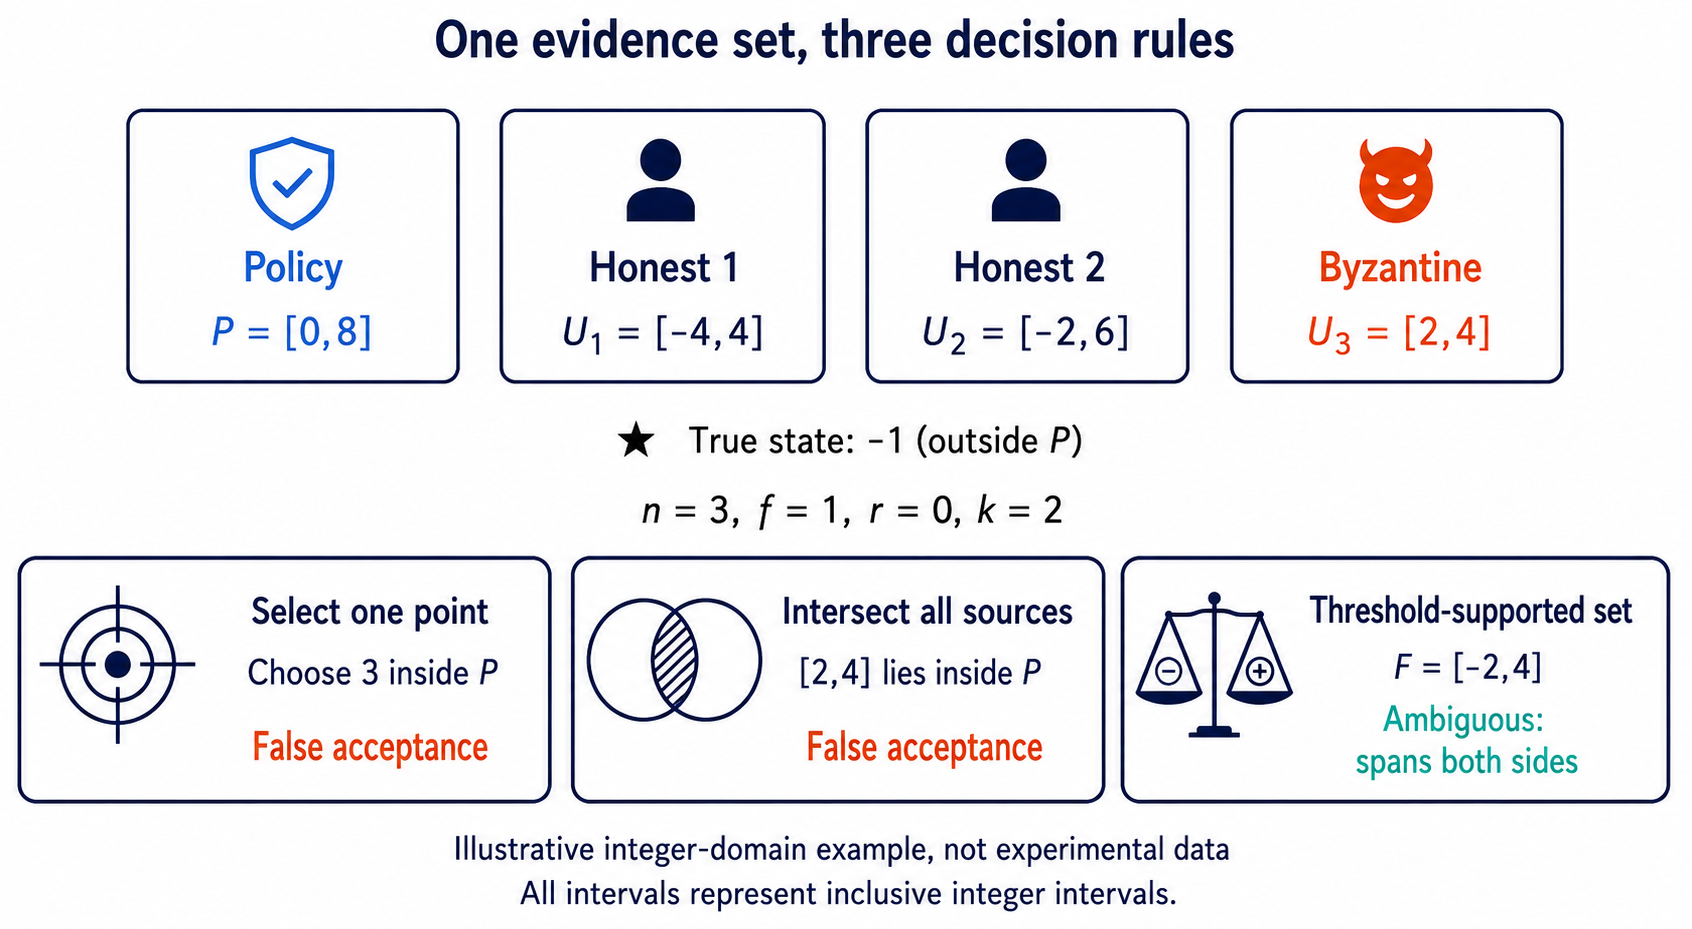
\includegraphics[width=\linewidth]{../figures/decision_counterexample.png}
\caption{Three rules applied to the same signed evidence, with inclusive integer intervals and $(n,f,r,k)=(3,1,0,2)$. A selected point or full-source intersection can falsely accept the known noncompliant true state, whereas threshold support yields an ambiguous decision. The example is constructed rather than measured.}\label{fig:counterexample}
\end{figure}

\subsection{Report binding and challenge--response verification}
The four-valued rule defines the evidence--policy relationship, but a geometric proof by itself cannot prevent the proof from being carried over to a different report or task. The prototype therefore uses the expiring challenge--response flow in Figure~\ref{fig:sequence}.

An administrator configures the task, verifying key, spacetime policy, threshold, and ordered issuer roster. The gateway retains a trusted snapshot of these settings and rejects repeated keys or trust-domain labels. It then generates a random 256-bit challenge $\nu$ using a trusted application clock and assigns an expiry time $e$. The vehicle and issuers derive a shared context:
\begin{equation}\label{eq:context}
c=\operatorname{OS2IP}\!\left(\operatorname{SHA256}\!\left(
\operatorname{Encode}(v,T,\nu,e,\operatorname{SHA256}(R))
\right)\right)\bmod q.
\end{equation}
Here $v$ is the protocol version, $T$ is the configured task, $R$ is the report's original byte sequence, $q$ is the BN254 scalar-field modulus, and $\operatorname{OS2IP}$ maps a byte sequence to an integer. Context $c$ binds the signed evidence and proof statement to a specified report and challenge. It neither encrypts the report nor hides its contents.

The implementation uses a Go JSON structure with fixed field order and no map fields. The report's SHA-256 digest is written as lowercase hexadecimal, and the issuer public-key byte arrays follow Go JSON's Base64 encoding. This defines deterministic bytes for the present prototype, not a standardized cross-language canonicalization. Implementations in other languages must reproduce the exact serialized bytes or agree upon a separately specified canonical format.

Each issuer signs a message digest containing $c$ and its measured interval. After collecting all signatures required by the roster, the vehicle applies Section~3.2's decision rule and constructs a zero-knowledge proof $\pi$ with interval endpoints and signatures as private witness data. The gateway checks the challenge's existence and validity period, reconstructs the public inputs from its trusted task snapshot and received report bytes, and checks the proof together with its decision code. It accepts only a proven Valid decision.

A successful verification atomically marks the nonce as used inside the current gateway instance. In the concurrent test with eight copies of one valid request, only one is accepted. Failed proof verification leaves an unexpired challenge available for legitimate retries; nevertheless, repeated invalid submissions can exhaust verification resources, so rate limiting is needed in deployment. The prototype neither persists nonce state across restarts nor implements distributed atomicity across gateway replicas. New nonces also do not, on their own, prevent resubmission of identical business reports.
\begin{figure}[htbp]\centering
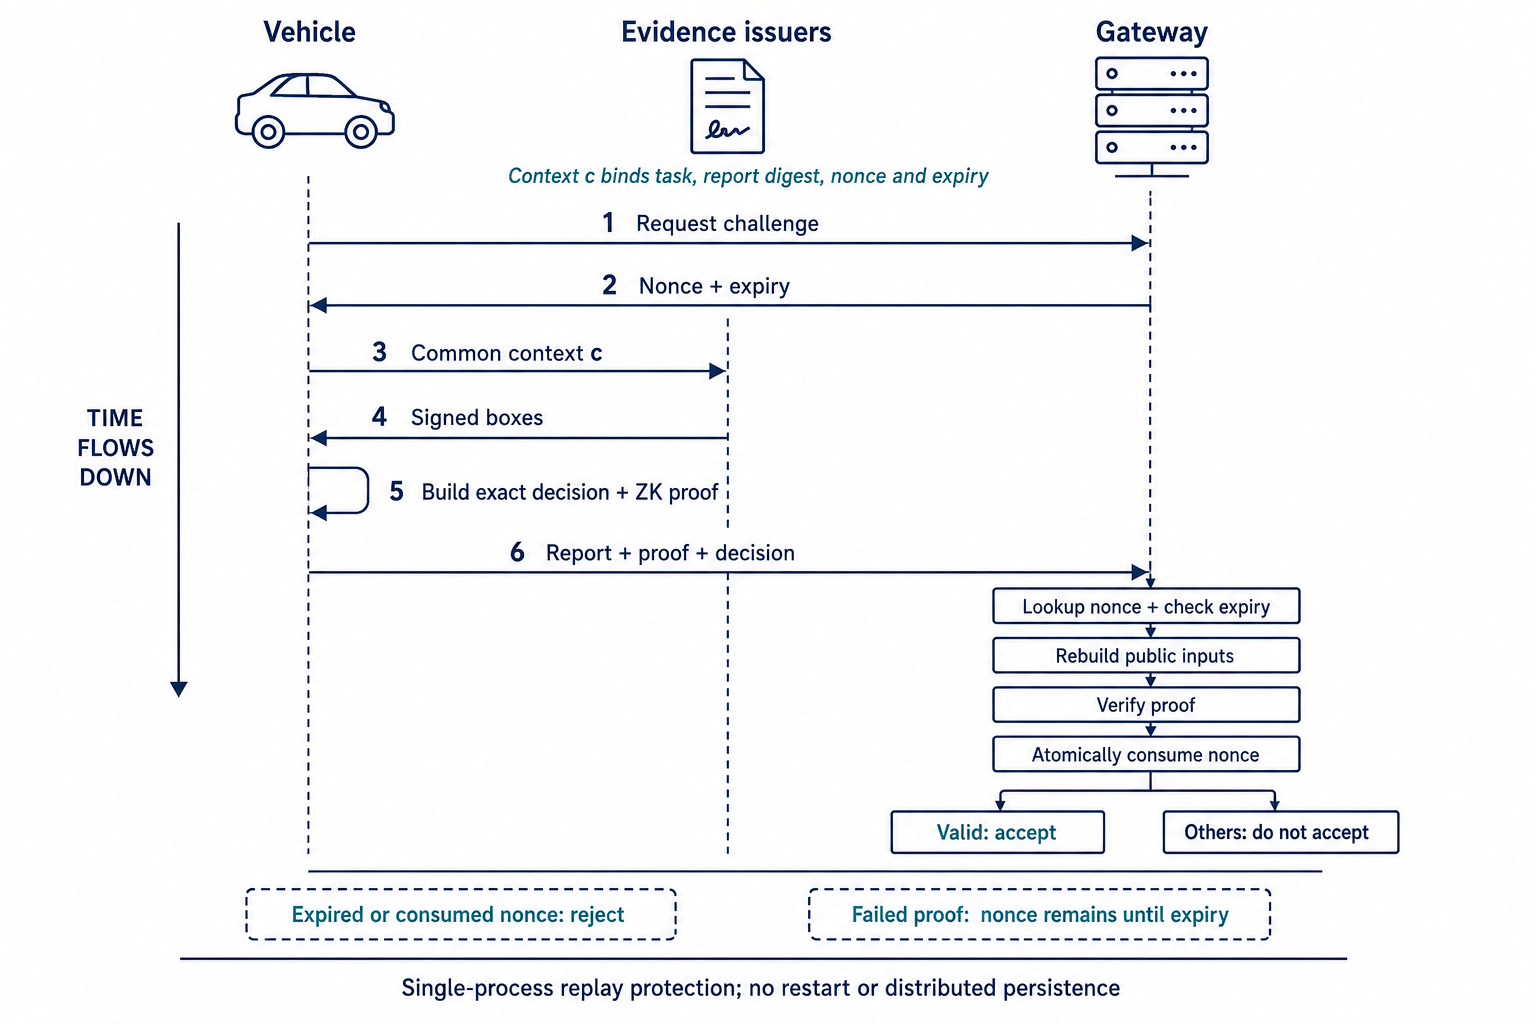
\includegraphics[width=\linewidth]{../figures/protocol_sequence.png}
\caption{Report-bound challenge and verification flow. After successful proof verification the gateway atomically marks the nonce as used within its current instance; failed attempts leave the challenge available for retries until expiry. Network transport details are omitted.}\label{fig:sequence}
\end{figure}

\subsection{Zero-knowledge circuit construction}
To certify a four-valued decision without revealing the original observations, the circuit checks signatures, coordinate bounds, and context consistency while determining whether threshold-supported states exist on either side of the policy boundary. We implement two geometric backends: lower-corner maximum-depth reachability and threshold-subset enumeration. Their signature-verification and public-output constraints are shared; they differ in how threshold reachability is calculated.

\subsubsection{Lower-corner maximum-depth reachability}
For a query box $Q\subseteq\Omega$, first clip every evidence box $U_i$ to $Q$. For each axis $a$, let $A_a$ contain the lower endpoints of the nonempty clipped boxes. The following lemma reduces maximum-depth search over the entire query region to a finite candidate set.

\begin{lemma}[Lower-corner maximum-depth reachability]\label{lem:corner}
If the maximum overlap depth inside $Q$ is positive, then some point attaining that depth belongs to $A_1\times\cdots\times A_d$.
\end{lemma}
\begin{proof}
Choose a point $z\in Q$ with maximum depth and let $\mathcal S$ be the collection of clipped boxes containing $z$. Their intersection is nonempty. For each axis $a$, define $v_a$ as the greatest lower endpoint of the boxes in $\mathcal S$. This endpoint belongs to $A_a$. Because $z$ belongs to every box in $\mathcal S$, the greatest lower endpoint on any axis cannot exceed the smallest corresponding upper endpoint. Hence $v=(v_1,\ldots,v_d)$ lies in every box in $\mathcal S$ and has depth at least $|\mathcal S|$, the maximum depth attained by $z$. By maximality, its depth is exactly the same. Thus $v$ is a maximum-depth point in the stated candidate set.
\end{proof}

By the lemma, the circuit enumerates at most $n^d$ lower-corner combinations, including duplicates, and checks both membership in $Q$ and coverage by the signed evidence boxes. A point with coverage at least $k$ exists in $Q$ if and only if an enumerated candidate meets that threshold. A candidate contributed by an interval not intersecting $Q$ cannot automatically be treated as valid: the necessary membership tests still apply.

When $P$ is an axis-aligned integer box, $\Omega\setminus P$ is the union of at most $2d$ axial slabs. Along axis $a$, a lower slab ends at $p_a^- -1$ and an upper slab starts at $p_a^+ +1$; all other axes span the discrete domain. Slabs lying outside $\Omega$ are inactive. The circuit calculates $I$ from reachability in $P$ and $O$ from the disjunction of reachability over complement slabs. It then constrains the public decision code to
\begin{equation}\label{eq:decisioncode}
\delta=(1-I)O+2IO+3(1-I)(1-O).
\end{equation}
For Boolean $I$ and $O$, this expression is exactly the coding in Table~\ref{tab:decisions}. Further constraints check the coordinate bit width, ordering of lower and upper endpoints, and containment of boxes and policy within $\Omega$. EdDSA/MiMC signatures are verified inside the circuit, and issuer public keys are compared for pairwise distinctness using their actual encoded elliptic-curve representations, rather than treating a public key as a single scalar.

\subsubsection{Threshold-subset enumeration and computational cost}
An alternative representation of the robust feasible set is
\begin{equation}\label{eq:subset}
\mathcal F_k=\bigcup_{\substack{S\subseteq[n]\\ |S|=k}}
\left(\bigcap_{i\in S}U_i\right),\qquad [n]=\{1,\ldots,n\}.
\end{equation}
The intersection of $k$ axis-aligned integer boxes is another box or the empty set. Its lower and upper endpoints are calculated by coordinatewise maxima and minima, making it possible to test nonemptiness, intersection with $P$, and existence of states outside $P$. Both the native reference implementation and the second circuit backend use this exact identity, with principal geometric work $O\!\left(\binom nk kd\right)$.

The advantages of the backends depend on the parameters. For fixed dimension, lower-corner reachability requires approximately $O((2d+1)d n^{d+1})$ geometric comparisons, in addition to signatures and $O(n^2)$ pairwise key-distinctness checks. Because $k$ is not fixed during circuit compilation, the same circuit shape can accept an admissible threshold as a public input. In contrast, subset enumeration fixes $k$ at compile time and constrains it against the public threshold. If the omission allowance $b=n-k=f+r$ is a small constant, its geometric work is $O(n^{b+1}d)$; when $k$ approaches $n/2$, the number of subsets instead grows combinatorially. These bounds characterize the geometric operations rather than the full cryptographic R1CS.

For example, at $(n,d,k)=(5,3,4)$, subset enumeration checks only $\binom54=5$ intersections, whereas lower-corner reachability checks up to $5^3=125$ candidates per query region. For an approximate comparison of parameter trends, define work proxies $W_D=(2d+1)d n^{d+1}$ and $W_S=\binom nk kd$. At $(20,3,19)$ they equal $3{,}360{,}000$ and $1{,}140$; when the threshold decreases to $10$, $W_D$ stays fixed while $W_S$ rises to $5{,}542{,}680$. These proxies count different types of operations and omit implementation constants, so their ordering cannot be interpreted as measured R1CS counts or proving time. The current experiments support subset enumeration only in the tested small-omission regime, not as a universal optimum.

Both circuits implement the same four-valued relation but trade threshold flexibility against geometric complexity. The prototype selects the backend explicitly; it does not switch between them automatically. The next section analyzes the security guarantee under the stated cryptographic and physical coverage premises.

\section{Security Analysis}\label{sec:security}
The preceding section defined the robust compliance relation and its realization in a zero-knowledge circuit. This section addresses what gateway acceptance can establish. Two related but distinct layers must be considered. Signatures, context binding, and zero-knowledge proofs constrain the origin of the submitted evidence, its association with a task, and the correctness of the computed relation. Inferring the position of the physical event from that evidence additionally requires coverage by honest sources. We specify the threat model, establish conditional soundness, and examine protocol attacks and information leakage.

\subsection{Threat model and security objectives}
We treat the vehicle and its communication network as untrusted. A computationally bounded adversary may intercept, modify, reorder, or replay reports, proofs, decision codes, and challenge parameters. It may use the legitimate private keys of compromised issuers to construct deceptive, policy-aware uncertainty regions. Honest issuers protect their signing keys and bind their observations to the intended event and task context. The gateway's authorized task configuration, verifying key, issuer roster, and clock are assumed trusted; signatures, hashes, and proof systems satisfy the stated computational security assumptions.

An issuer identity is a logically authorized unit defined by enrollment and trust-domain configuration. The gateway can detect repeated keys or trust-domain identifiers, but this check alone does not establish independence of real institutions or confer Sybil-resistant registration. Likewise, an authenticated signature does not imply physical measurement accuracy. Witness confidentiality is primarily defined against the protocol verifier: zero knowledge does not disclose private spacetime boxes and their signatures, but it does not hide an issuer's measurements from that issuer or conceal the business report and network metadata.

We examine six properties: evidence authenticity, context integrity, conditional acceptance soundness, witness confidentiality, challenge freshness, and fail-closed behavior. Table~\ref{tab:security-properties} links each to its assumptions and implemented checks. Source availability, physical sensor calibration, Sybil-resistant enrollment, anonymous transport, cross-task unlinkability, and privacy under unrestricted adaptive policy queries are beyond the present proof relation.

\begin{table}[htbp]\centering\footnotesize
\caption{Security properties, prerequisites, and validation.}\label{tab:security-properties}
\begin{tabularx}{\linewidth}{@{}p{0.20\linewidth}p{0.30\linewidth}X@{}}\toprule
Property & Assumptions & Mechanism or observation\\\midrule
Evidence authenticity & Honest keys uncompromised outside the Byzantine allowance; signature unforgeability & In-circuit EdDSA/MiMC verification; modified signed bounds rejected\\
Context integrity & Trusted task configuration; signed-message and context mappings satisfy collision/binding assumptions & Binding to task, report, roster, threshold, nonce and expiry; tested substitutions rejected\\
Conditional acceptance soundness & Sound proof system; at most $f$ Byzantine issuers and $r$ honest misses & Four-valued relation, Propositions~\ref{prop:soundness}--\ref{prop:composition}, and synthetic checks tagged by $M\le r$\\
Witness confidentiality & Zero knowledge of the instantiated proof system; explicit public-output leakage & Box endpoints and signatures remain private witness values; other disclosure is summarized in Table~\ref{tab:privacy-boundary}\\
Freshness & Trusted clock; atomic challenge updates in one gateway instance & Expiry checks and atomic marking after successful verification; one accepted among eight concurrent replays\\
Fail-closed behavior & Correct gateway procedure and complete configured roster & Missing/malformed evidence, mismatched codes, unknown/expired challenges, or duplicated roster entries abort or are rejected\\\bottomrule
\end{tabularx}\end{table}

The principal limitation is that a valid cryptographic proof does not imply an accurate physical measurement. A compliance decision about the true event follows only when enough honest observations actually cover that event.

\subsection{Correctness and conditional soundness}
\begin{proposition}[Conditional evidence soundness]\label{prop:soundness}
Suppose at most $f$ of the $n$ enrolled issuers are Byzantine, and at most $r$ boxes submitted by honest issuers fail to cover the same true reference state $z^\star$. With $k=n-f-r$, we have $z^\star\in\mathcal F_k$. Consequently, a Valid decision entails $z^\star\in P$, and an Invalid decision entails $z^\star\notin P$.
\end{proposition}
\begin{proof}
At least $n-f-r=k$ honest boxes contain $z^\star$. By the definition of the feasible set in~\eqref{eq:feasible}, its coverage depth is at least $k$, so $z^\star\in\mathcal F_k$. A Valid decision requires $\varnothing\ne\mathcal F_k\subseteq P$, implying $z^\star\in P$. An Invalid decision requires $\mathcal F_k\cap P=\varnothing$, implying $z^\star\notin P$.
\end{proof}
This is the standard threshold-containment argument under the explicit fault and coverage assumptions, not a new interval-fusion theorem. If the additional inequality $n>2f+r$ holds, then $k>f$, so every threshold-supported state has at least one honest supporter. That stronger condition is not needed to show that the true state belongs to $\mathcal F_k$. Neither conclusion makes every feasible state the true state or guarantees that a signed physical error bound is properly calibrated.

To quantify potential failure of the coverage premise, let $\mathcal H$ be the set of honest issuers, and let $M$ count honest boxes that miss $z^\star$. For the stated operating population, suppose issuer $i\in\mathcal H$ has a marginal miss probability at most $\alpha_i$. Even without independence between sources,
\begin{equation}\label{eq:calibration}
\Pr(M>r)\le \min\!\left\{1,\frac{\sum_{i\in\mathcal H}\alpha_i}{r+1}\right\}.
\end{equation}
Indeed, $\mathbb E[M]\le\sum_{i\in\mathcal H}\alpha_i$, and $M>r$ implies $M\ge r+1$; the bound follows from Markov's inequality for a nonnegative integer-valued variable. This generally loose bound allows dependent errors but supplies no missing calibration measurements. Adaptive choice of tasks or policies requires applicable conditional calibration or a joint bound; marginal failure rates estimated on unrelated samples cannot be used without justification. A Poisson--binomial tail may be sharper if independent Bernoulli misses are justified, but shared positioning bias commonly invalidates that assumption.

Moving from authenticated evidence to gateway acceptance also requires computational security. Under knowledge soundness of the instantiated Groth16 proof system, an accepted proof implies at least one witness assignment satisfying the circuit's signature, range, and geometric constraints. Signature unforgeability for authorized keys, the required binding properties of the MiMC signed-message prehash and context mapping, and correct reconstruction of public inputs associate that witness with authenticated evidence for the designated task and report. The witness need not be unique, and the existence of its signatures does not authenticate the physical truth of the measurements.

Groth16 additionally requires a circuit-specific trusted setup. Exposure of trapdoor values that must remain secret can compromise knowledge soundness. The setup used in our benchmarks serves only the experiment. Deployment requires appropriate parameter generation, potentially with multiple independent participants, or a different proof-system setup model followed by renewed security and performance evaluation.

\begin{proposition}[Gateway acceptance under physical coverage]\label{prop:gateway}
Assume the task and keys are authorized; the gateway procedure and clock are trustworthy; honest-issuer signatures are unforgeable; the proof system is knowledge sound; and the MiMC message prehash and context mapping satisfy the required collision and binding properties. If the gateway accepts a report and the fault and coverage conditions of Proposition~\ref{prop:soundness} hold, then its report-bound reference event satisfies the configured policy $P$, except in the event of a stated cryptographic failure.
\end{proposition}
\begin{proof}
The gateway reconstructs the public statement from its trusted task snapshot and the received report bytes. It accepts only a verified proof with decision code Valid. Under the stated assumptions, verification establishes the existence of signed boxes satisfying that statement. Substitution of an honest issuer's box or its context while retaining authentication would require a failure of the relevant signature, digest binding, or proof-system guarantee. The valid classification enforces $\varnothing\ne\mathcal F_k\subseteq P$. Under the physical coverage premise, Proposition~\ref{prop:soundness} gives $z^\star\in\mathcal F_k$, hence $z^\star\in P$.
\end{proof}
The proposition concerns the location of the reference event bound to the report, not the truth of every factual claim in the report payload. It also assumes that honest issuers generated their evidence for the same event and context. Equation~\eqref{eq:calibration} can be used to discuss physical-premise failure only when its calibration assumptions apply; this prototype has not established a field-calibrated guarantee for real multisource vehicular evidence.

To separate computation security from physical assumptions, write $\mathsf{Acc}$ for gateway acceptance, $\mathsf{Cov}$ for the event that both the Byzantine and honest-miscoverage allowances hold, and $\mathsf{Comp}$ for the event that the report-bound true reference state lies in the authorized policy. For the chosen adversary resources and concrete parameters, let $\varepsilon_{\rm snark}$, $\varepsilon_{\rm sig}$, $\varepsilon_{\rm MiMC}$, $\varepsilon_{\rm ctx}$, and $\varepsilon_{\rm state}$ upper-bound failures, respectively, of the proof-system soundness guarantee, required signature unforgeability, signed-message prehash binding, deterministic context-map binding, and challenge-state enforcement.

\begin{proposition}[Composed conditional acceptance bound]\label{prop:composition}
Under trusted task configuration, roster, and gateway clock, and with the failure events defined above,
\begin{equation}\label{eq:composed}
\Pr[\mathsf{Acc}\land\mathsf{Cov}\land\neg\mathsf{Comp}]
\leq \varepsilon_{\rm snark}+\varepsilon_{\rm sig}
+\varepsilon_{\rm MiMC}+\varepsilon_{\rm ctx}+\varepsilon_{\rm state}.
\end{equation}
\end{proposition}
\begin{proof}
Suppose none of the stated cryptographic or state checks fails. An accepted proof then has a witness satisfying the configured task, report, roster, threshold, nonce, expiry, and signature constraints. Its Valid classification implies $\varnothing\ne\mathcal F_k\subseteq P$. Under $\mathsf{Cov}$, Proposition~\ref{prop:soundness} establishes $z^\star\in\mathcal F_k$, and hence $\mathsf{Comp}$. Thus occurrence of $\mathsf{Acc}\land\mathsf{Cov}\land\neg\mathsf{Comp}$ requires at least one of the enumerated failures. Applying the union bound yields~\eqref{eq:composed}.
\end{proof}

The bound concerns \emph{wrong acceptance while the physical coverage premise holds}; it is not the unconditional false-acceptance rate in deployment. An unconditional guarantee also requires estimating the probability and relevance of $\neg\mathsf{Cov}$. In the modeled single-process gateway without restart, atomic marking after successful verification prevents a second acceptance of the same challenge; the corresponding term for this specific replay behavior can be taken as $\varepsilon_{\rm state}=0$. No such zero-failure claim extends to process restarts, multiple gateways, or every possible state-management fault.

The prototype uses 256-bit challenge nonces, SHA-256 for report and context digests, Groth16 over BN254, and the BN254 twisted-Edwards EdDSA/MiMC implementation provided by gnark. This EdDSA instantiation is not Ed25519. The analysis composes stated assumptions but does not re-prove the cryptographic library or collapse its heterogeneous primitives into one overall security-bit estimate. Cryptography certifies authenticated evidence and its computation; physical coverage determines whether the result applies to the real event.

\subsection{Resistance to protocol attacks}
We first consider evidence tampering and context substitution. Changing the bounds of a signed region changes its message under~\eqref{eq:signedbox}, so, assuming signature security, it cannot pass in-circuit verification while retaining an honest issuer's original signature. Replacing the task, report, roster, threshold, challenge, or expiry changes the public statement reconstructed by the gateway. A proof made for a previous statement cannot simply be submitted for a different one without violating the relevant signature, digest-binding, or proof-system assumption. Missing evidence, malformed rosters, and incorrect decision codes lead to rejection or abort, not to a proved Inconsistent classification.

Challenge replay is checked by validating the nonce and expiry, verifying the proof, and atomically recording successful use. This prevents an already accepted nonce from authorizing another request within the same implemented gateway instance. The observed acceptance of one among eight concurrent replay copies is consistent with this guarantee. Failed verification does not consume an unexpired nonce so that legitimate retries remain possible. An attacker can therefore submit invalid proofs repeatedly to consume verification capacity; rate limits, resource quotas, persistent state, and distributed consistency must be supplied by the deployment. Nor does a fresh nonce automatically detect resubmission of the same report.

Finally, consider Byzantine sources that select their intervals strategically with knowledge of the public policy. Provided the Byzantine and honest-miscoverage budgets hold, Proposition~\ref{prop:soundness} gives $z^\star\in\mathcal F_k$ irrespective of malicious box placement. A true event outside $P$ therefore cannot yield a Valid feasible set wholly inside $P$, while a true event inside $P$ cannot yield an Invalid feasible set wholly outside it. Malicious sources may nevertheless reduce the frequency of decisive outcomes or withhold signatures and force abort. No corresponding guarantee follows if either budget or the honest coverage assumption fails. Our synthetic attacks use true-state and policy-boundary information to choose adversarial boxes, but they are not a substitute for adversarial evaluation in a deployed system.

The current protocol addresses evidence authentication, context integrity, and same-instance challenge replay. It does not ensure continuous issuer availability, resistance to denial of service, revocation, or dynamic operation with a partial roster; those protections require additional system mechanisms.

\subsection{Privacy boundary and information leakage}
Zero knowledge enables verification of the four-valued relation without exposing the issuer boxes and signatures that constitute the private witness. It does not hide all protocol information. In this implementation the gateway receives report bytes $R$ and combines them with the task and challenge fields to reconstruct public context $c$. Therefore $c$ is a deterministic binding value, not encryption of $R$ or a hiding commitment. If the report comes from a small enumerable space and the remaining context fields are available, an observer who sees $c$ may recompute candidate digests and perform an offline dictionary test. The gateway, which receives $R$ directly, cannot obtain report confidentiality from the proof's zero-knowledge property.

\begin{table}[htbp]\centering\footnotesize
\caption{Visibility and leakage boundaries for protocol participants.}\label{tab:privacy-boundary}
\begin{tabularx}{\linewidth}{@{}p{0.19\linewidth}p{0.37\linewidth}X@{}}\toprule
Role & Visible within the protocol model & Not concealed by the ZK guarantee\\\midrule
Evidence issuer & Its own observation and region, signing operation, and report-bound context & Its own evidence and any report data supplied by the host application\\
Vehicle/prover & Report, regions, and signatures required to build the witness & Secrecy of the witness from the prover itself is not an objective\\
Gateway/verifier & Report bytes, task/domain, policy, threshold, roster, nonce/expiry, public context, proof, classification & Report content, public policy, issuer identities, classification\\
Public transcript observer & Exposed statement, proof, classification, and transport metadata & Linkability of public fields and offline candidate tests for low-entropy reports\\\bottomrule
\end{tabularx}\end{table}

The four-valued classification itself reveals information. If only $q$ such outputs are considered, they admit at most $4^q$ different sequences and thus at most $2q$ bits of discrete output entropy. This counts the output alphabet only; it excludes information conveyed by other public fields and is not a location-privacy guarantee. If an attacker can adapt the spatial policy and observe subsequent classifications, the feedback may progressively reduce the candidate location region. The amount of leakage depends on policy geometry, query privileges, and prior information; no fixed localization accuracy or convergence rate follows merely from the $2q$ bound.

The prototype protects private witnesses only under an authorized, challenge-bound policy-query model. Unrestricted adaptive querying, network anonymity, hidden roster membership, and cross-business unlinkability are not provided. Applications requiring repeated location checks or stronger identity privacy must add external policy authorization and auditing, query-rate or budget controls, and suitable transport and identity protections.

\section{Experimental Evaluation}
We evaluate the proposed evidence-certification method along three axes: protocol behavior, decision semantics, and cryptographic cost. First, we manipulate the evidence, task context, and challenge parameters to determine whether the implementation handles invalid inputs as specified. We then control the true state, measurement errors, and Byzantine participation in synthetic workloads to assess the scope of the four-valued decision rule and compare it with alternative methods. Finally, we measure the proving costs of both Groth16 circuit backends and examine scalability alongside a public location-proof implementation and a resource-constrained compilation study. The tests evaluate distinct aspects of the protocol, finite model, and implementation; they do not constitute an end-to-end vehicle deployment.

\subsection{Implementation and experimental setup}
\subsubsection{Cryptographic implementation and test environment}
The prototype is implemented in Go 1.25.6 using gnark 0.14.0~\cite{gnark}, Groth16 over BN254~\cite{Groth2016}, and gnark's EdDSA/MiMC primitives for signing evidence and verifying signatures inside the circuit~\cite{MiMC2016}. The signature curve is \texttt{tedwards.BN254}, not Ed25519. Key generation, signing, parameter setup, proving, and verification all execute actual cryptographic implementations. BN254 was chosen for a reproducible prototype and benchmark; it is neither a post-quantum security claim nor a validated long-term deployment choice. The source and experiment scripts are maintained in the implementation repository. Its identifying link is omitted from this review copy; the source paths \texttt{prototype/} and \texttt{experiments/} refer to that repository's root.

Proof benchmarks ran on a Mac mini with an eight-core Apple M1 processor and 16 GB of memory. For each circuit configuration, one experimental setup was followed by 30 proofs and verifications using a fixed valid signed witness. Reported proving times exclude circuit compilation, evidence acquisition, network transport, queueing, and energy consumption. For context, we also implemented a simplified hidden-point region-membership circuit on the same gnark/Groth16/BN254 stack. Without issuer authentication, threshold fusion, or four-valued decisions, this circuit is a structural point of reference rather than a functionally equivalent baseline.

To examine circuit size separately from proving time, we compiled signed-evidence R1CS instances at issuer counts $n\in\{4,8,12,16\}$ and dimensions $d\in\{2,3\}$. For each pair we evaluated subset circuits with $k=n-1$, $k=n-2$, and $k=n/2$, along with the corresponding lower-corner circuit, for 32 compilation invocations in total. Each run had a 30-second timeout, a termination threshold of 3 GiB sampled resident set size (RSS), and a 2500 MiB Go soft memory target. We do not impute constraint counts to resource-limited runs. This experiment measures compilation feasibility and size, not proof latency at the largest configurations.

\subsubsection{Synthetic evidence and trajectory replay}
The semantic study uses the three-dimensional integer domain $\Omega=[0,63]^3$ and policy $P=[18,45]^3$. It configures five issuers, Byzantine budget $f=1$, and baseline honest-miscoverage allowance $r=0$. The design crosses maximum uncertainty radii $\{2,4,6\}$, actual Byzantine counts $\{0,1,2\}$, and three error models (independent calibrated, correlated calibrated, and undercovered), yielding 27 conditions. Each condition contains 30 random seeds and 80 events per seed, or 64,800 base observations in total. Three quarters of the events are placed near a policy face to emphasize boundary decisions. Honest interval radii are drawn from the ranges specified for each condition. Byzantine sources select their regions adversarially using the true state and public policy rather than only introducing random perturbations.

We compare the robust feasible-set rule with a median point claim, majority-center voting, a fixed maximum-radius margin, and all-source intersection. False acceptance (FA) uses truly noncompliant events as its denominator; false rejection (FR) uses truly compliant events. \emph{Decisive coverage} is the fraction of all events classified Valid or Invalid, excluding Ambiguous and Inconsistent decisions. It measures the frequency of definite answers, not their accuracy. When a seed has no events for a class-specific denominator, we do not assign an arbitrary zero error rate. Randomized equivalence tests also compare the native subset classifier, lower-corner search, and exhaustive classifier on tested inputs. The semantic workload uses the native classifier and does not generate a full Groth16 proof for every synthetic event; cryptographic timing is obtained from separate measurements.

Each event records $M$, the number of honest intervals that fail to cover the true state $z^\star$, allowing explicit checks of Proposition~\ref{prop:soundness}'s premise $M\le r$. To isolate threshold effects, the same 64,800 observations are re-evaluated with $r\in\{0,1,2\}$. This gives 194,400 \emph{paired evaluations}, not 194,400 new independent observations.

For trajectory replay, we extract 787 measured reference states spanning 786 seconds from UrbanNav-HK-Medium-Urban-1~\cite{UrbanNav}. After transformation to a local integer coordinate frame, a fixed percentile-defined policy includes 169 of the states. Each of 30 replay runs simulates four honest evidence sources, one policy-aware Byzantine source, and bounded correlated errors along the measured path. A stress mode multiplies the common-mode bias by four. The reference motion is measured; the multisource uncertainty boxes are simulated. This experiment therefore does not demonstrate that a real multisensor positioning system satisfies the physical coverage assumption.

\subsection{Protocol-security regression tests}
Table~\ref{tab:security-validation} records adversarial tests against the implemented proof-and-gateway path. Mutations target the evidence, decision code, context, issuer roster, and challenge nonce. The purpose is to check whether the implementation enforces the constraints from Sections~3 and~4, not to assess the physical accuracy of sensors.

\begin{table}[htbp]\centering\small
\caption{Adversarial regression tests of proof generation and gateway verification.}\label{tab:security-validation}
\begin{tabularx}{\linewidth}{@{}p{0.22\linewidth}p{0.35\linewidth}X@{}}\toprule
Attack & Enforced constraint & Observed prototype response\\\midrule
Evidence-bound tampering & Signed interval endpoints, issuer slot, context & Altered signed bounds were rejected\\
Decision substitution & Agreement between four-valued circuit output and public decision code & Tested mismatched proof/code pairs were rejected\\
Task or report substitution & Binding to task, report, threshold, roster, nonce and expiry & Tested cross-context substitutions were rejected\\
Challenge replay & Expiry and atomic state update after successful verification & Unknown or expired nonces were rejected; one of eight concurrent copies succeeded\\
Roster manipulation & Distinct ordered keys and trust-domain labels & Duplicated keys or labels were rejected\\
Missing issuer evidence & Complete evidence from the provisioned roster is required & Protocol aborted rather than certifying inconsistency\\\bottomrule
\end{tabularx}\end{table}

The results show that a proof associated with a different task or report cannot be transplanted directly into the current public statement, and missing roster data are not misreported as semantic inconsistency. The eight-way replay test supports only the implemented single-instance, no-restart guarantee of atomically marking a successfully used nonce. It does not establish distributed gateway safety, persistence across restarts, or business-report deduplication.

\subsection{Robustness and baseline comparison}
Across 12 synthetic conditions in which the actual Byzantine count and the generated honest coverage meet their specified allowances, the robust rule produced no observed wrong decisive classifications. Its mean decisive coverage was 87.52\%, compared with 75.63\% for the fixed-margin rule. These are observations under controlled assumptions, not estimates of failure rates in an actual vehicular deployment.

Table~\ref{tab:semantic} gives the focus condition, which uses calibrated correlated errors, maximum radius four, and one Byzantine issuer. The robust rule makes a decisive classification in 85.04\% of events, compared with 75.67\% for fixed margins. A median-point rule decides every event but produces 2.10\% false acceptance and 15.29\% false rejection. All-source intersection yields a high rate of evidence failure and can also make incorrect decisions, illustrating why requiring every source to agree is not inherently robust to adversarial observations.

\begin{table}[htbp]\centering\small
\caption{Focus-condition classification results: means over 30 seeds of 80 events each (percent). FA/FR use outside/inside denominators; the other columns use all events.}\label{tab:semantic}
\begin{tabular}{lrrrrr}\toprule
Method&FA&FR&Amb.&Failure&Decisive\\\midrule
Median point claim&2.10&15.29&0&0&100\\
Majority center&2.10&16.30&0&0&100\\
Fixed maximum-radius margin&0&0&24.33&0&75.67\\
All-source intersection&8.64&47.55&0&87.63&12.38\\
Robust feasible set&0&0&14.96&0&85.04\\\bottomrule
\end{tabular}\end{table}

A paired bootstrap with 10,000 resamples, using each random seed's paired outcomes as the resampling unit, estimates a 9.38-percentage-point increase in decisive coverage for the robust rule over fixed margins. The 95\% bootstrap percentile interval is 8.25--10.54 percentage points. This interval describes the difference for the specified synthetic workload; it is not a confidence statement about the population of real-world road conditions.

To check the theorem's premise explicitly, we group outcomes by the number $M$ of honest boxes that miss the true state. In the focus condition, all 2,400 events satisfy $M=0$, and no wrong decisive result was observed. Events sharing one random seed may be dependent, however, so 2,400 event records are not treated as independent trials proving a zero population error rate. Taking each seed's group of 80 events as one unit, and treating the presence of at least one wrong decisive result within that group as a Bernoulli failure, zero failures in 30 independent seed groups gives a one-sided 95\% exact binomial upper bound of 9.50\% on the group-level failure probability. That bound still applies only to the fixed synthetic generator.

Under the undercoverage error model, the fractions of events satisfying $M\le r$ are 52.42\%, 62.79\%, and 73.42\% for $r=0,1,2$, respectively. No wrong decisive classifications were observed among those satisfying the premise. Among events with $M>r$, the corresponding wrong-decisive rates were 1.31\%, 0.67\%, and 0.47\%. These diagnostics show that errors \emph{may} occur when the sufficient premise of Proposition~\ref{prop:soundness} is violated; they do not establish that every such violation causes an error, nor do they estimate the frequency of physical-premise failure in the field.

\begin{figure}[htbp]\centering
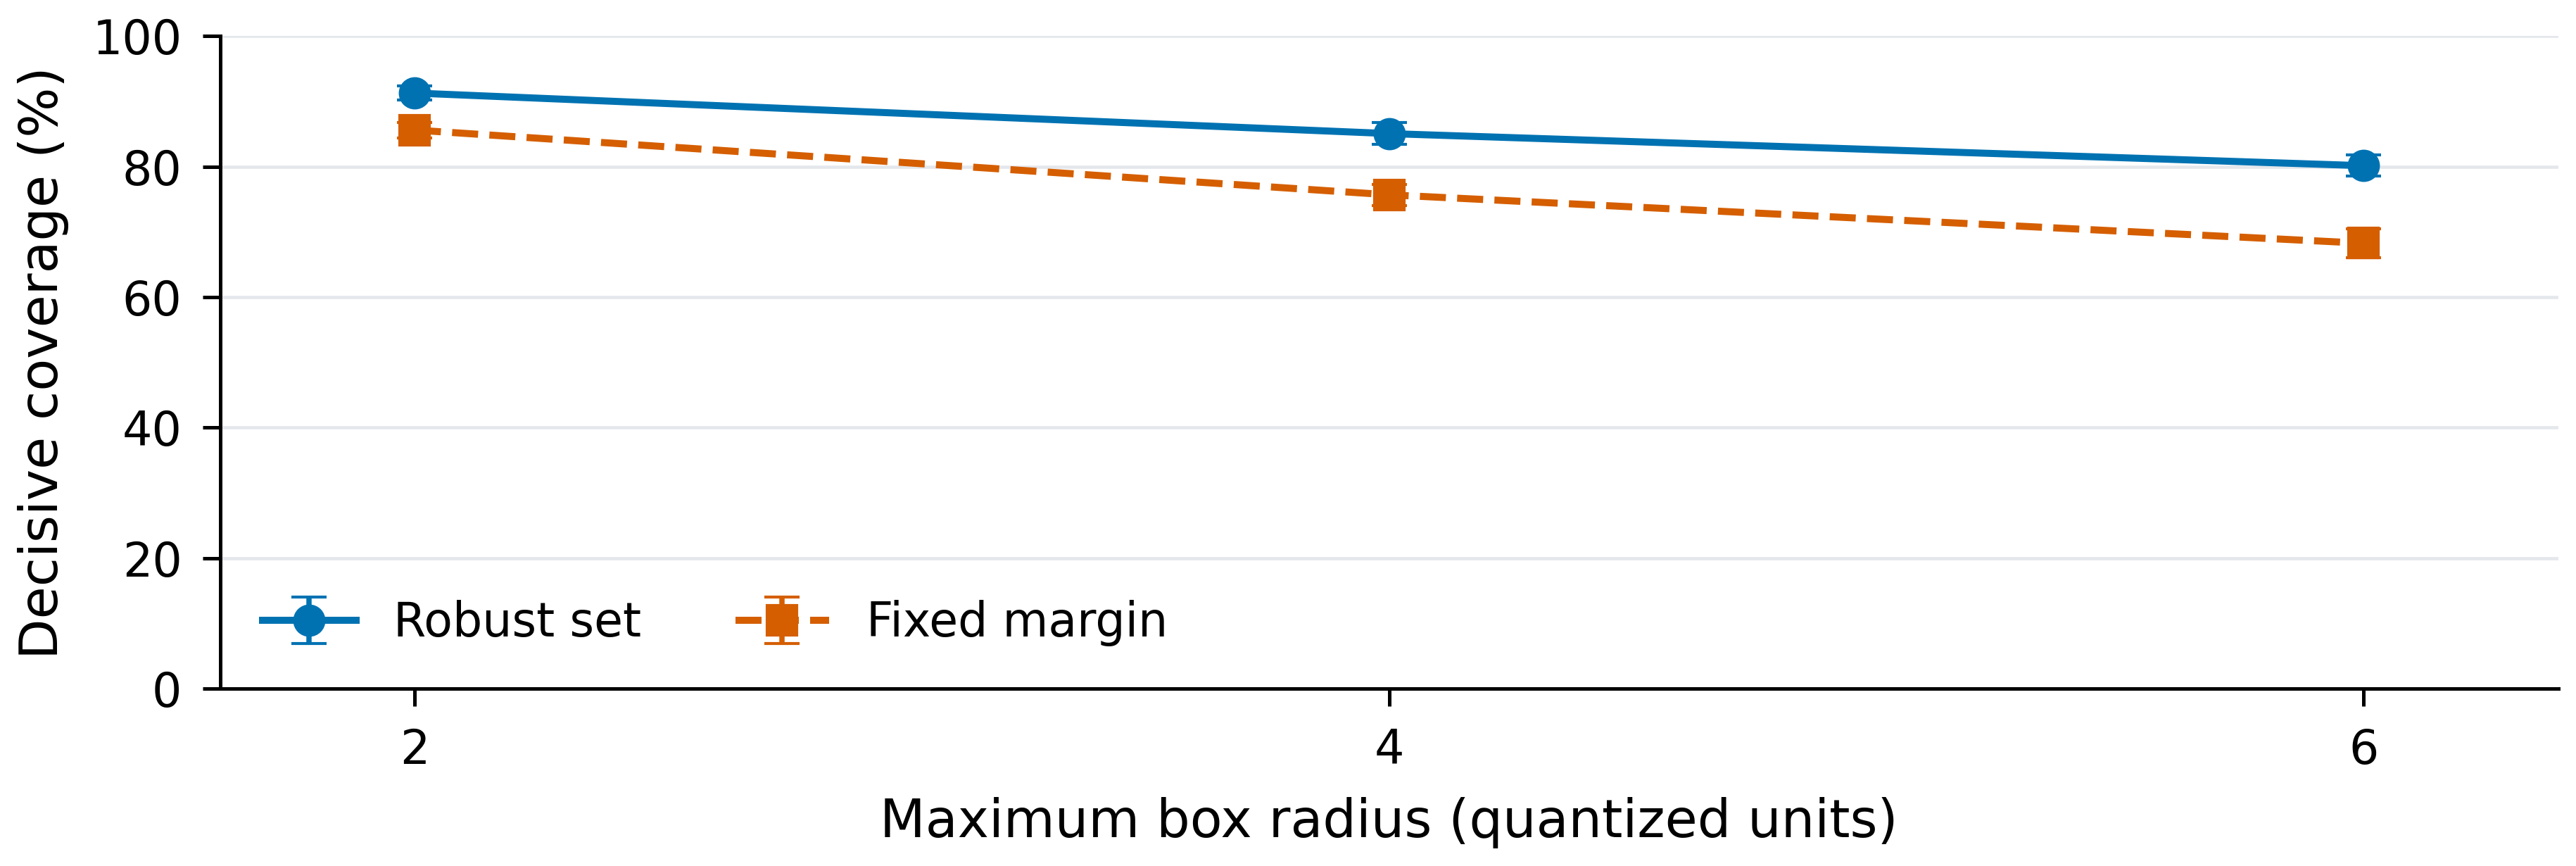
\includegraphics[width=\linewidth]{../figures/availability.png}
\caption{Decisive coverage versus maximum uncertainty radius for correlated calibrated errors with one Byzantine issuer. Error bars are normal-approximation 95\% intervals over 30 seed-level rates. Radius is expressed in quantized units, not calibrated physical distance.}\label{fig:availability}
\end{figure}

\subsection{Ablation and out-of-budget stress tests}
Table~\ref{tab:assumption-stress} examines two distinct violations of the stated assumptions. Honest-source undercoverage can produce wrong decisive results even when the number of Byzantine issuers remains within $f=1$. When two issuers are Byzantine but the verifier still assumes a budget of one, false acceptance, false rejection, and evidence failure all rise markedly. Inconsistent evidence therefore denotes an empty threshold-supported set, not a general detector of every fault-budget or calibration violation.

\begin{table}[htbp]\centering\small
\caption{Stress conditions violating source assumptions: means over 30 seeds (percent).}\label{tab:assumption-stress}
\begin{tabularx}{\linewidth}{@{}Xrrrr@{}}\toprule
Condition&FA&FR&Evidence failure&Decisive\\\midrule
Honest undercoverage; Byzantine count within budget&0.23&3.41&0&84.92\\
Two actual Byzantine issuers with verifier budget $f=1$&11.62&60.86&83.33&16.67\\\bottomrule
\end{tabularx}\end{table}

Table~\ref{tab:miscoverage} varies the allowed honest miscoverage $r$ while holding the observed evidence fixed. Under calibrated evidence, increasing $r$ from zero to two lowers decisive coverage from 85.04\% to 77.46\%, without observed wrong decisive decisions. For undercovered evidence, a larger $r$ accompanies a reduction in false rejection from 3.41\% to 0.94\%, while decisive coverage falls from 84.92\% to 78.50\%. With $n$ and $f$ fixed, increasing $r$ reduces $k=n-f-r$ and expands $\mathcal F_k$. It is then harder for \emph{every} feasible state to lie within the authorized policy. Thus changing the allowance alters decision conservatism but does not improve physical sensor calibration.

\begin{table}[htbp]\centering\small
\caption{Paired ablation over honest-miscoverage allowance ($n=5$, $f=1$, maximum radius four, one Byzantine issuer; percent).}\label{tab:miscoverage}
\begin{tabular}{lrrrr}\toprule
Error model&$r$&FA&FR&Decisive coverage\\\midrule
Calibrated&0&0&0&85.04\\
Calibrated&1&0&0&81.25\\
Calibrated&2&0&0&77.46\\
Undercovered&0&0.23&3.41&84.92\\
Undercovered&1&0&1.79&81.67\\
Undercovered&2&0&0.94&78.50\\\bottomrule
\end{tabular}\end{table}

\begin{figure}[htbp]\centering
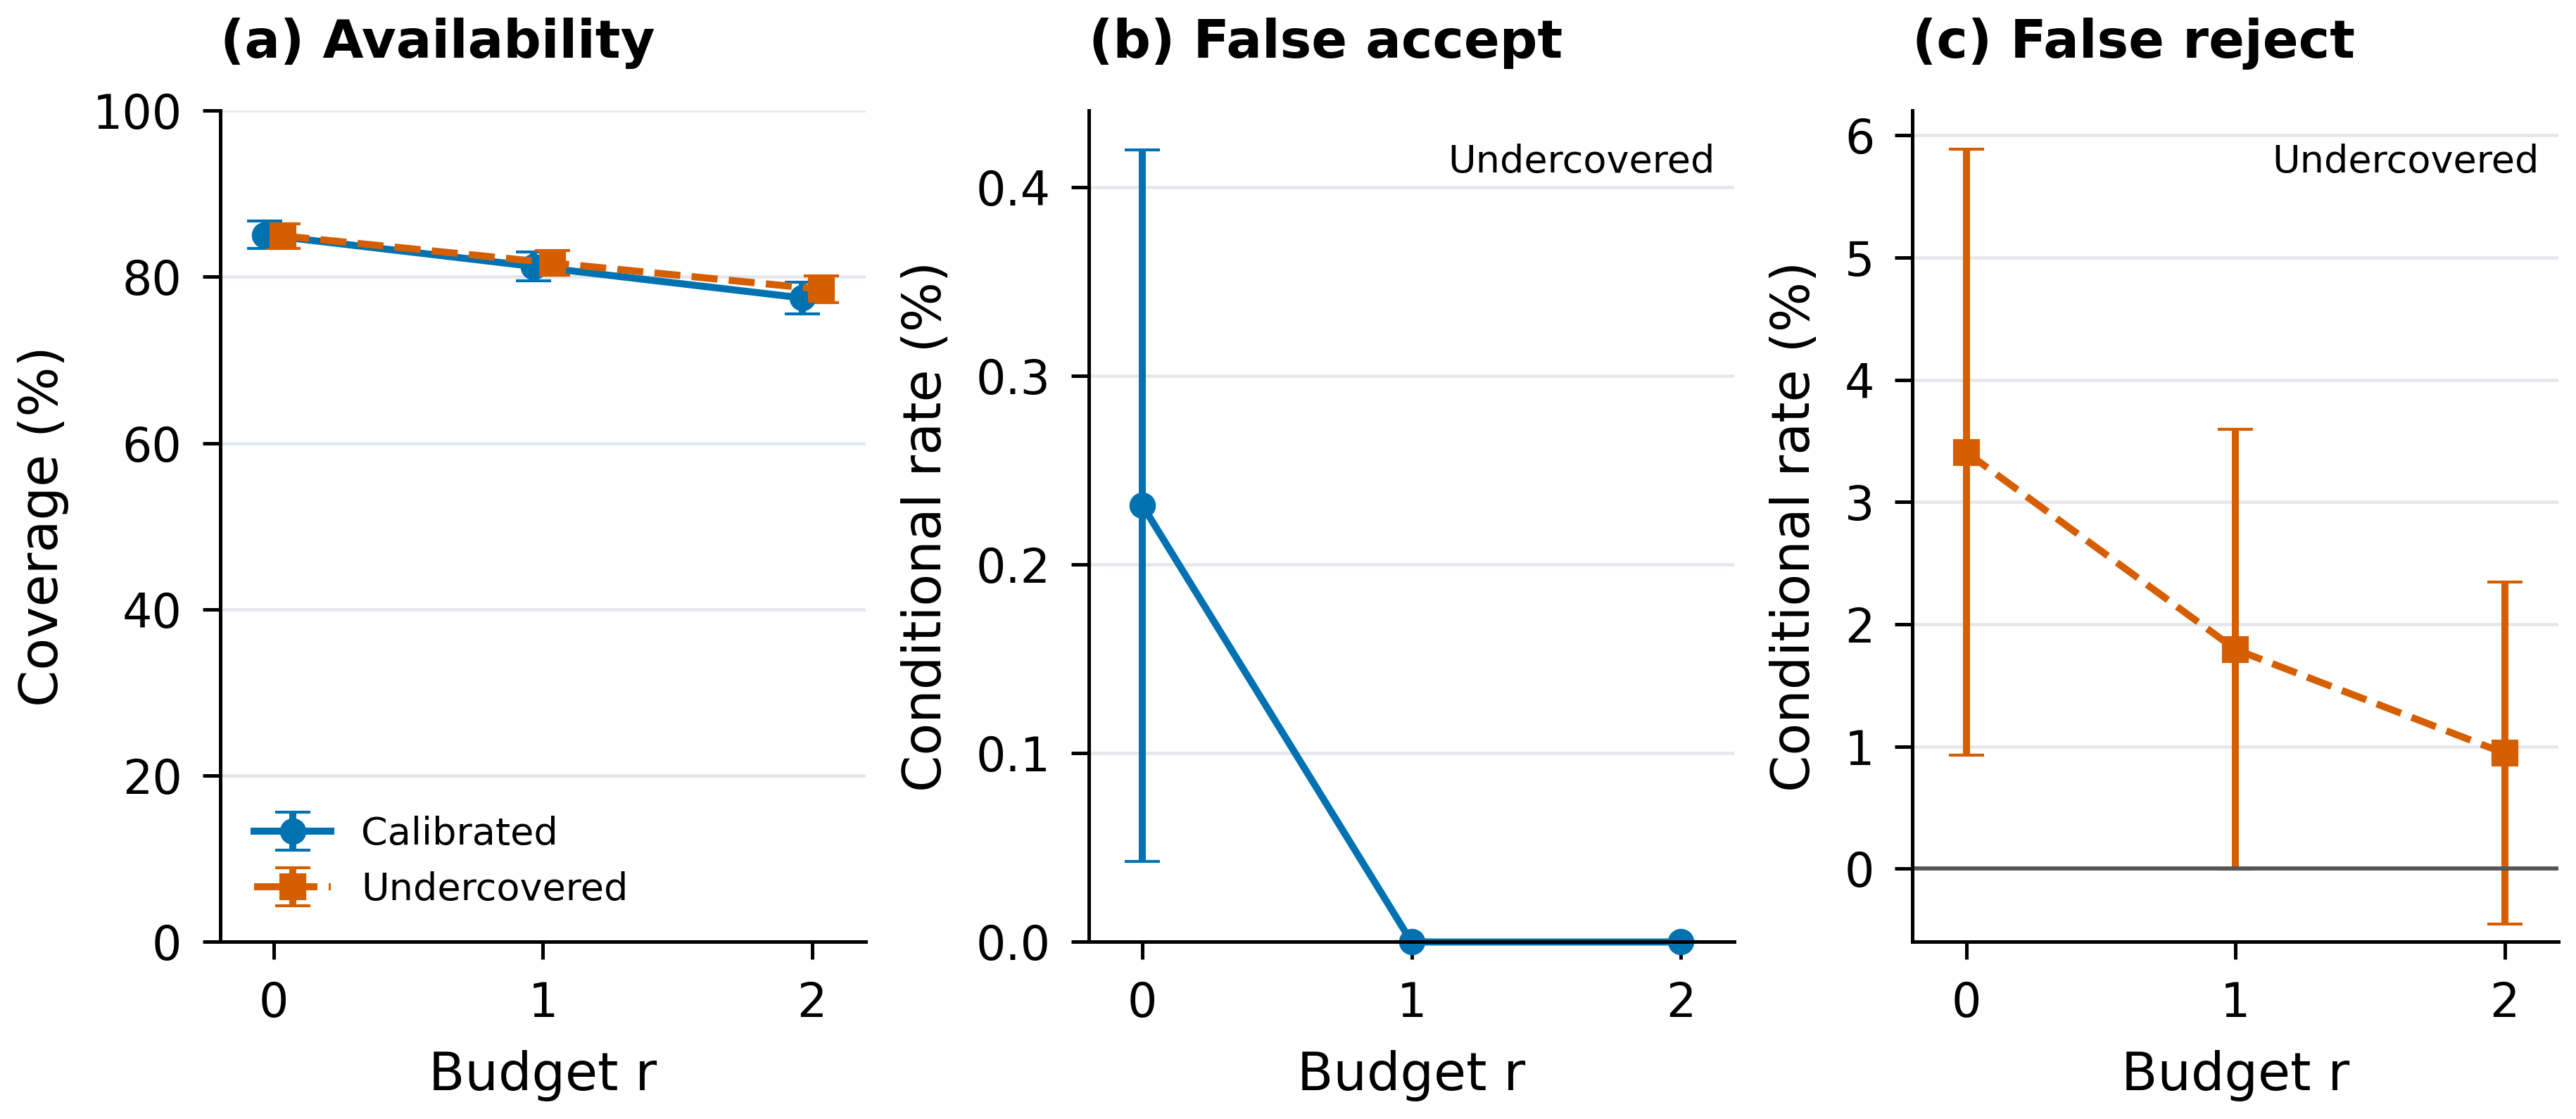
\includegraphics[width=\linewidth]{../figures/budget_tradeoff.png}
\caption{Effects of the honest-miscoverage allowance $r$ for $n=5$, $f=1$. Points are means over the same 30 seeds; error bars are normal-approximation 95\% intervals. Zero-width intervals for observed zero errors do not imply a population error probability of zero; occasional negative plotted interval endpoints arise from the normal approximation.}\label{fig:budget}
\end{figure}

Replay over a measured reference path provides a complementary test. With nominal simulated evidence along UrbanNav, the robust rule achieves 93.27\% decisive coverage, compared with 81.94\% for fixed margins; neither produced observed errors. The median-point rule has 0.29\% false acceptance and 3.12\% false rejection. When the simulated common-mode bias is multiplied by four, the robust rule exhibits 0.032\% false acceptance and 0.493\% false rejection. All of these figures describe simulated evidence on a measured trajectory, not calibration of real multisensor hardware. In particular, the 77.46\% value in Table~\ref{tab:miscoverage} belongs to the synthetic $r=2$ ablation, not to UrbanNav under common-mode bias.

\subsection{Comparison with recent related work}
Table~\ref{tab:recent-context} places the evaluation in the context of representative work published or released between 2024 and 2026. The table records the scale and selected findings reported by the respective authors, with particular attention to what each system verifies. Hardware, interaction models, cryptographic libraries, and security relations differ, so source-reported times cannot be converted into a common performance ranking.

\begin{table}[htbp]\centering\footnotesize
\caption{Selected quantitative findings from recent systems and the boundaries of comparison. Values are reported by the cited sources.}\label{tab:recent-context}
\begin{tabularx}{\linewidth}{@{}p{0.17\linewidth}p{0.24\linewidth}X@{}}\toprule
Method&Evaluation scale&Reported outcome and methodological boundary\\\midrule
BFT-PoLoc~\cite{BFTPoLoc} (2024)&Up to 450 challengers&At 450 challengers, roughly 45\% of localization uncertainty was below 100 km and 95\% below 1000 km; Byzantine network localization rather than a zero-knowledge policy proof\\
PG~\cite{PG} (2024)&261 cloud nodes; 19 constrained sensors&Private Byzantine-tolerant fusion using distributed garbled circuits, with an output-delivery guarantee\\
ZKLP~\cite{ZKLP} (2025)&Floating-point location SNARK&Proximity proof about 0.26 s and verification throughput about 470 peers/s; geometric properties of a hidden point\\
Vehicle ZK-PoL~\cite{VehiclePolicy} (2025)&Up to 43,800 trajectory points&Electric-vehicle subsidy and highway compliance proofs about 36 min and 59 min; interactive, trajectory-scale setting\\
CRSF~\cite{CRSF} (2026)&Up to 261 sensors&Approximately one second for the measured phases at the largest instance; collusion-resistant private fusion rather than a policy certificate\\\bottomrule
\end{tabularx}
\end{table}

To reduce differences attributable to hardware, we also reproduced a fixed version of the publicly available ZKLP implementation. ZKLP was pinned to commit \texttt{e8e321524982} and its first ZKLP32 test vector was executed on the same GitHub Actions Ubuntu runner as our $(n,d)=(3,2)$ subset circuit. Both use Groth16/BN254 and were measured over ten proof generations after setup. However, ZKLP depends on a branch based on gnark v0.9.1, whereas our implementation uses gnark v0.14.0, and the proved relations are different. This is therefore a comparison under a shared runner, not a fully controlled experiment with identical libraries and predicates.

\begin{table}[htbp]\centering\small
\caption{Fixed-version ZKLP reproduction and subset circuit on the same runner (sample medians over ten post-setup proofs).}\label{tab:zklp-repro}
\begin{tabular}{lrrrrr}\toprule
Implementation&Constraints&Prove (ms)&Verify (ms)&Proof (B)&Public witness (B)\\\midrule
Pinned ZKLP32&19,467&515.53&1.739&196&140\\
Our subset $(3,2)$&32,474&645.14&1.547&164&556\\\bottomrule
\end{tabular}
\end{table}

ZKLP mainly proves geometric predicates of a hidden coordinate. Our corresponding circuit additionally checks three signed uncertainty intervals, issuer roster and context constraints, threshold support, and a four-valued classification. Its larger circuit and public witness therefore include additional authentication work; their difference cannot be attributed exclusively to geometric-algorithm efficiency. An older \texttt{m6i.xlarge} record in the ZKLP repository reports 21,878 constraints and 270.03 ms median proving time, while the pinned code compiles to 19,467 constraints in the current environment. The records alone do not isolate the effects of version, hardware, or configuration, and we do not interpret the difference as a performance trend.

\subsection{Cryptographic performance and circuit scalability}
\subsubsection{Structural reference using a simplified relation}
Table~\ref{tab:point-zk} reports a hidden-point region-membership circuit on the same cryptographic stack. It contains only a test of whether a private point belongs to the public policy; it omits issuer signatures, interval uncertainty, Byzantine budgets, threshold fusion, and four-valued output. It is therefore a reference for the cost of a weaker relation, not a functionally matched baseline.

\begin{table}[htbp]\centering\small
\caption{Simplified hidden-point membership circuit with 16-bit bounds under Groth16/BN254.}\label{tab:point-zk}
\begin{tabular}{rrrr}\toprule
Dimension $d$&R1CS constraints&Proof (B)&Public witness (B)\\\midrule
2&408&164&268\\
3&612&164&396\\\bottomrule
\end{tabular}
\end{table}

By contrast, the smallest complete subset circuits contain 32,474 constraints at $(n,d)=(3,2)$ and 35,248 at $(3,3)$. Their additional constraints arise jointly from in-circuit signature verification, issuer-key and coordinate checks, context binding, threshold fusion, and the four-valued relation. They cannot all be attributed to robust geometry alone. In each tested configuration, a Groth16 proof occupies 164 bytes.

\subsubsection{Measured costs of the two geometric backends}
Tables~\ref{tab:crypto} and~\ref{tab:subset} report lower-corner and threshold-subset costs for matched small configurations. Each circuit is set up once and evaluated using 30 proofs. Figure~\ref{fig:scaling} displays the distribution of proving times. Public witness sizes span 556--748 bytes across the reported shapes, excluding report plaintext and transport framing.

\begin{table}[htbp]\centering\small
\caption{Lower-corner Groth16 measurements. Setup is in seconds; all other times are in milliseconds.}\label{tab:crypto}
\begin{tabular}{rrrrrrr}\toprule
$(n,d)$&Constraints&Setup&Prove p50&Prove p95&Verify p50&Verify p95\\\midrule
$(3,2)$&55,987&3.64&213.12&244.83&1.033&1.350\\
$(4,2)$&97,493&7.47&360.74&427.17&1.081&1.514\\
$(5,2)$&158,781&11.56&574.69&700.49&1.073&1.212\\
$(3,3)$&185,229&13.84&548.33&707.35&1.067&1.412\\
$(4,3)$&510,362&38.34&1090.95&1212.54&1.093&1.506\\\bottomrule
\end{tabular}
\end{table}

\begin{table}[htbp]\centering\small
\caption{Threshold-subset Groth16 measurements for $k=n-1$ (times in milliseconds).}\label{tab:subset}
\begin{tabular}{rrrr}\toprule
$(n,d)$&Constraints&Prove p50&Verify p50\\\midrule
$(3,2)$&32,474&163.42&1.028\\
$(4,2)$&42,918&225.79&1.038\\
$(5,2)$&53,528&254.66&1.051\\
$(3,3)$&35,248&206.34&1.059\\
$(4,3)$&46,737&234.93&1.038\\\bottomrule
\end{tabular}
\end{table}

\begin{figure}[htbp]\centering
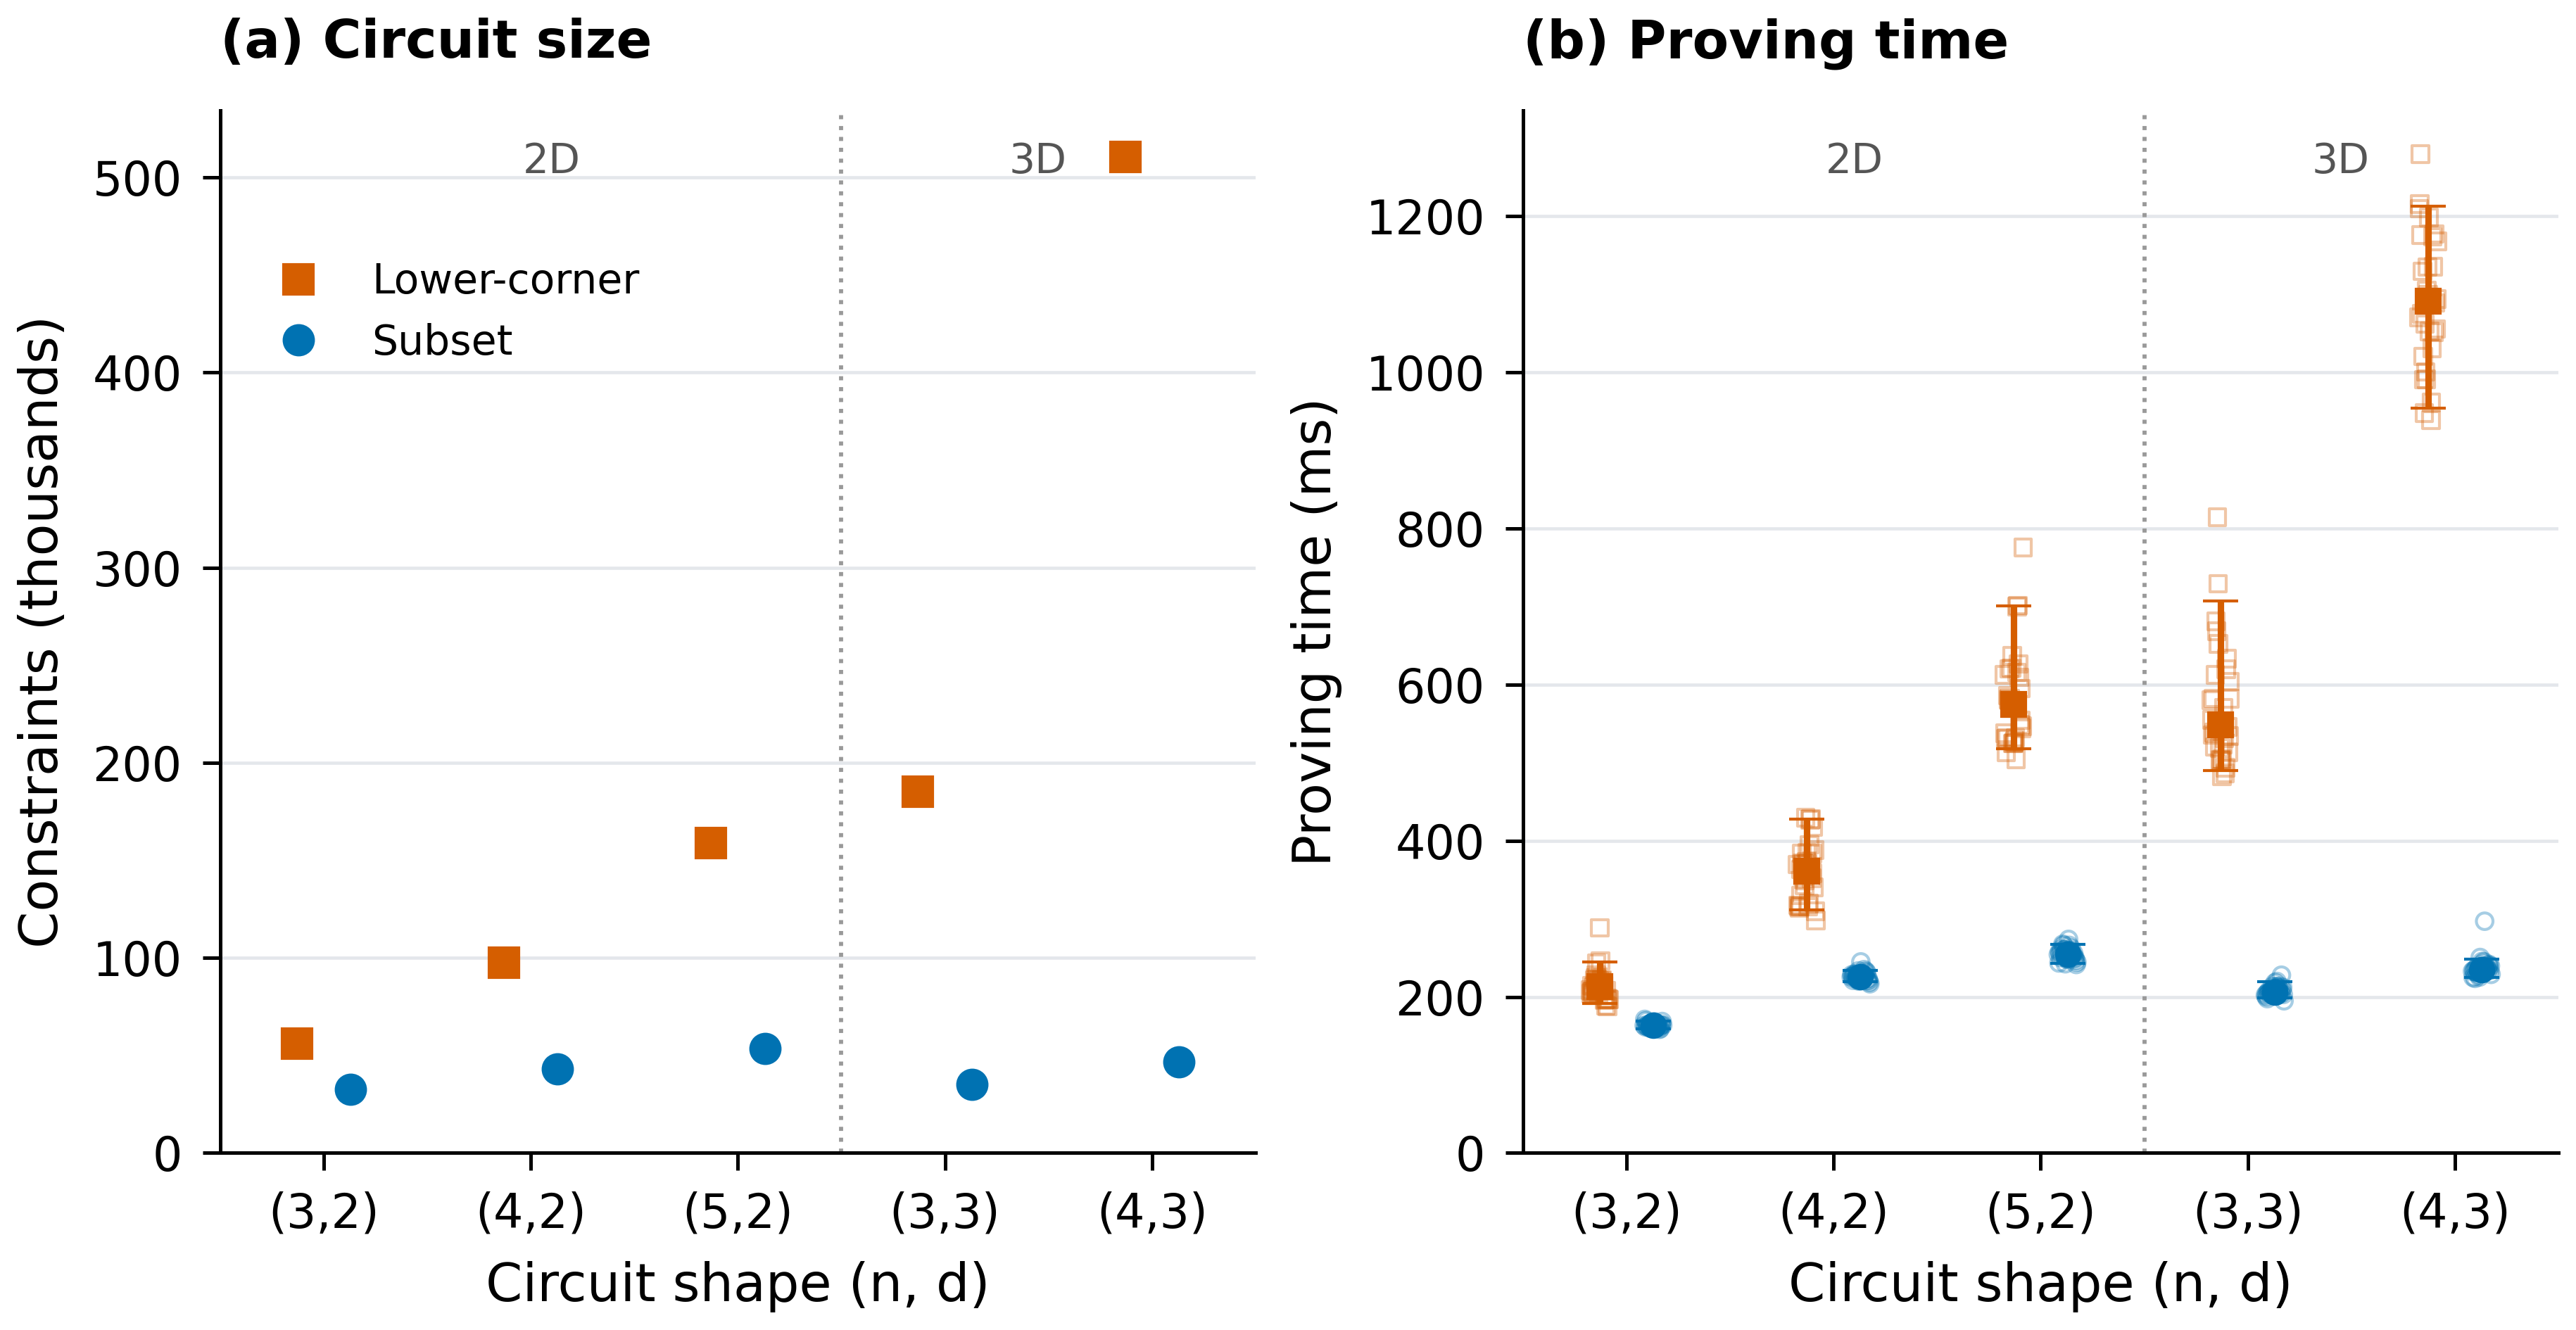
\includegraphics[width=\linewidth]{../figures/backend_costs.png}
\caption{R1CS size and proving time for the two backends on the Apple M1 platform. Small points in the timing panel show all 30 observations per circuit shape and backend (300 total); large markers are medians and intervals span the empirical p5--p95 range, not confidence intervals. Backend batches were not interleaved.}\label{fig:scaling}
\end{figure}

Subset enumeration has fewer constraints in every tested configuration with $k=n-1$. For example, at $(n,d)=(4,3)$, lower-corner reachability requires 510,362 constraints and has a median proving time of 1090.95 ms; the subset backend requires 46,737 constraints and 234.93 ms. The observed ratio of approximately 4.64 is descriptive for the specified test platform, because the backend batches were not interleaved. It is not a universal speedup corrected for environmental variation, and smaller circuits do not by themselves establish the same advantage at every size.

\subsubsection{Resource-limited compilation scalability}
Figure~\ref{fig:compilegrowth} and Table~\ref{tab:compilegrowth} summarize 32 resource-bounded compilation invocations. Of these, 27 completed; five were terminated after the sampled RSS reached the 3 GiB threshold, indicated by \texttt{RL}. At $(d,n)=(2,16)$, lower-corner reachability has 3,509,645 constraints, compared with 181,194 and 308,978 constraints for subsets with omissions $b=n-k$ equal to one and two. At $(d,n,k)=(3,12,6)$, the balanced-threshold subset circuit already has 962,018 constraints. We do not assign estimated counts to unfinished builds or claim that they are theoretically uncomputable.

\begin{table}[htbp]\centering\small
\caption{Resource-limited R1CS compilation sweep with complete signature and geometric constraints. \texttt{RL} indicates termination before a count was obtained.}\label{tab:compilegrowth}
\begin{tabular}{rrrrrr}\toprule
$d$&$n$&Lower corner&Subset $b=1$&Subset $b=2$&Subset $k=n/2$\\\midrule
2&4&97,493&42,918&43,160&43,160\\
2&8&509,277&86,354&97,734&111,776\\
2&12&1,544,390&132,447&181,221&675,759\\
2&16&3,509,645&181,194&308,978&RL\\
3&4&510,362&46,737&47,099&47,099\\
3&8&RL&95,153&112,213&133,255\\
3&12&RL&147,506&220,640&962,018\\
3&16&RL&203,793&395,417&RL\\\bottomrule
\end{tabular}\end{table}

\begin{figure}[htbp]\centering
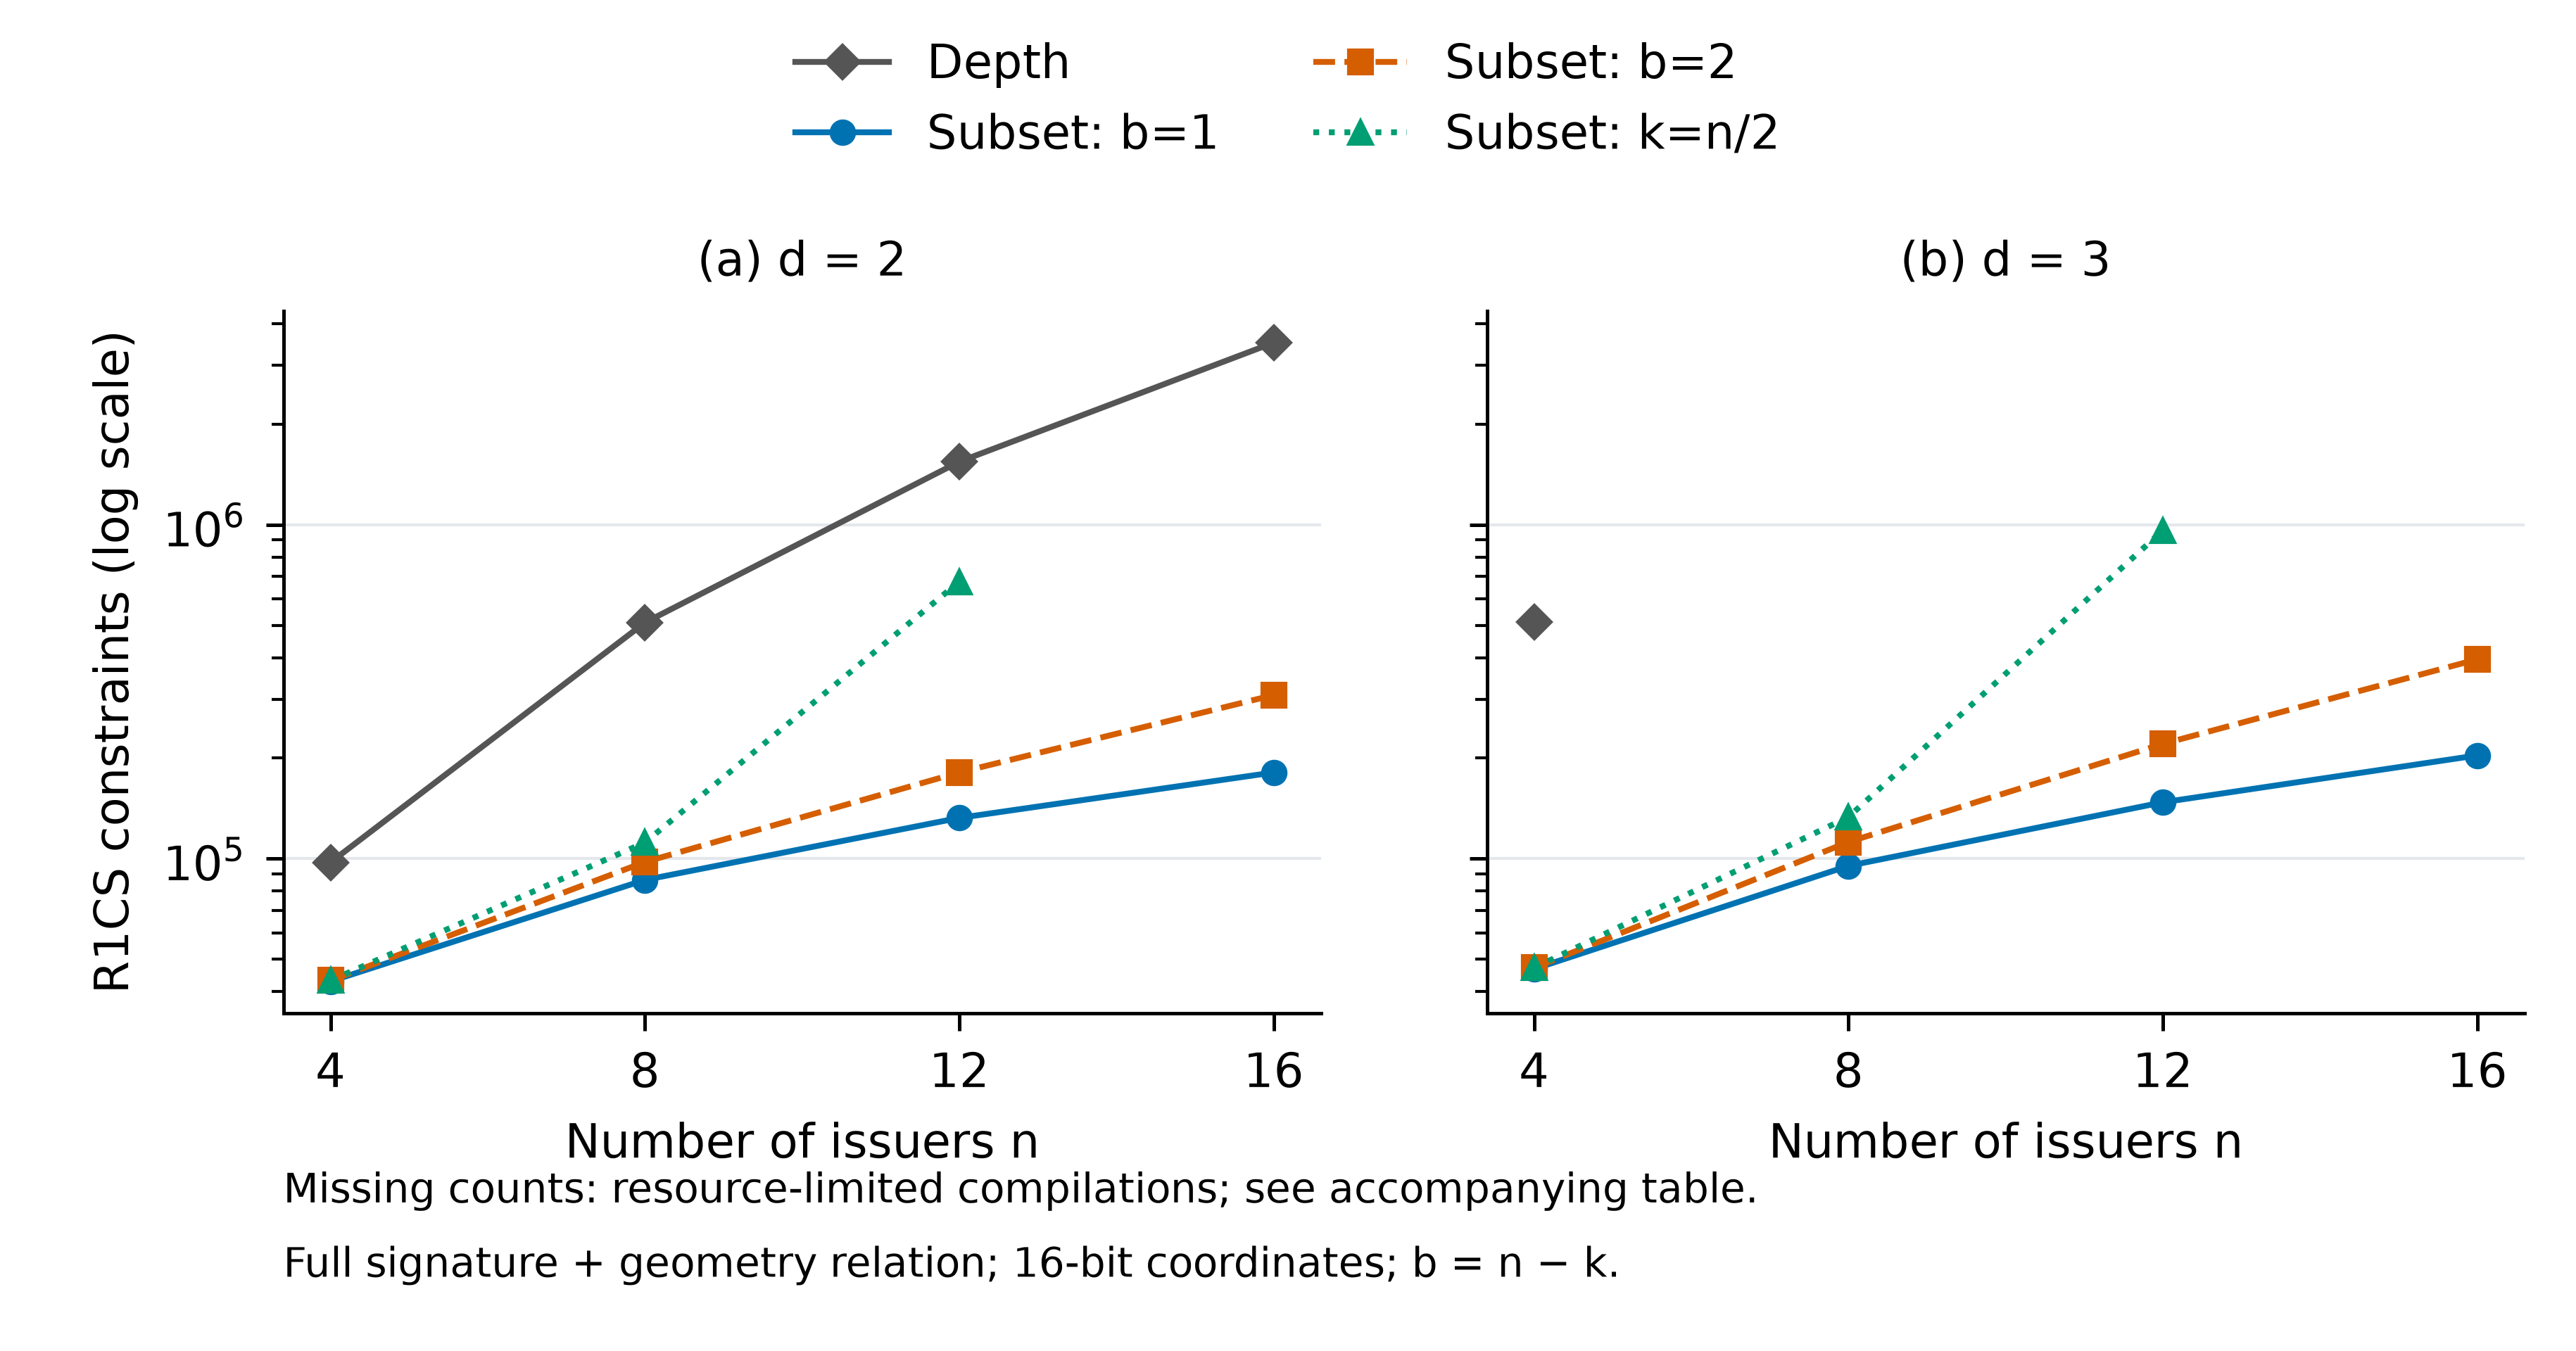
\includegraphics[width=\linewidth]{../figures/compile_scalability.png}
\caption{Resource-limited sweep of full R1CS constraint counts. Missing markers correspond to terminated compilations, not zero constraints; connecting lines are visual guides. These are compilation results, not large-circuit proving times.}\label{fig:compilegrowth}
\end{figure}

Taken together, the direct measurements and compilation results favor subset enumeration for the tested small omission budgets $b=f+r$. As $k$ approaches half the source count, however, the number of subsets $\binom nk$ grows rapidly and can diminish the advantage. The evidence supports backend selection for particular tested scales and thresholds, rather than a universal optimum across dimensions, source populations, and hardware.

\subsection{Discussion and system limitations}
The experiments support the correctness of the implemented finite-domain certification relation and its computational feasibility for the tested parameters. They do not replace field evaluation of a deployed vehicular crowdsensing system. The prototype is an evidence-certification component for a host application, not a complete platform for recruiting participants, assigning rewards, managing dynamic participation, or guaranteeing continuous service. A proof can certify the computation relating private signed intervals to a public policy; it cannot itself establish that those intervals were physically calibrated or that the report payload accurately describes a real event.

\emph{Physical coverage remains the central external premise.} The synthetic generator controls whether honest intervals cover the true state, while UrbanNav replay adds simulated multisource errors to a measured reference path. The retrospective single-receiver diagnostic in Appendix~\ref{app:receiver} illustrates a related risk: a fixed uncertainty envelope derived from a historical calibration segment contains 76 of 78 reference epochs in that segment but only 2 of 69 in a later evaluation segment. Because the sequence is temporally dependent and uses offline combined processing, the result is neither an independent-trial estimate of coverage nor evidence about real-time multisource positioning. It indicates that a static calibration bound may fail to transfer across operating periods. Real deployment requires verifiable calibration for each source and operating regime, together with investigation of common-mode biases.

\emph{System reliability depends on the fixed roster and gateway state.} A complete roster prevents a prover from arbitrarily dropping inconvenient pre-registered evidence, but a single issuer refusing to sign may force abort. Removing duplicate keys and trust-domain labels does not establish independent institutional control. Nonce-state persistence across restarts, atomic consistency across gateway instances, key revocation, duplicate-report suppression, and request rate limits must be implemented by the host system. Similarly, zero knowledge hides the signed-interval witness, not the plaintext report received by the gateway, the public policy and roster, or the four-valued classification. Enumerable report spaces and repeated adaptive policy queries can still disclose information.

\emph{The performance results have a specific platform scope.} We measure the proving kernel on an Apple M1 workstation and R1CS compilation under selected resource limits. We do not measure on-board-unit energy consumption, end-to-end vehicle-to-infrastructure latency, real multisource evidence-acquisition time, or sustained throughput. Groth16's circuit-specific trusted setup also requires secure deployment arrangements. Zero observed errors in calibrated synthetic cases must therefore be interpreted within the finite model and coverage assumptions, rather than as a reliability estimate for a vehicle in the field.

\section{Conclusion}
We have proposed zero-knowledge spacetime compliance certification over signed uncertainty evidence for vehicular crowdsensing with uncertain observations and Byzantine failures. Unlike verification of a single concealed coordinate, the method forms a robust feasible set of all states supported by at least $k=n-f-r$ sources, under explicit Byzantine allowance $f$ and honest-miscoverage allowance $r$. A four-valued rule checks the relationship between this set and the public policy, accepting a report only when the set is nonempty and wholly contained in the authorized region. This avoids treating an unsupported selected point or vacuous set inclusion as sufficient authorization evidence.

The relation is implemented through lower-corner reachability and threshold-subset enumeration circuits over Groth16/BN254, together with a gateway that binds verification to the task, report, and challenge. Protocol tests exercise signed-evidence tampering, context substitution, and reuse of the same challenge within a single gateway instance. Under the configured fault and coverage premises, the robust rule produced no observed wrong decisive outputs in calibrated synthetic tests; across 12 such conditions, mean decisive coverage was 87.52\%, compared with 75.63\% for fixed margins. The measured subset backend also has fewer constraints and shorter proving times in the tested small-omission configurations. These findings support implementation feasibility for the finite-domain evidence relation, but cannot be extrapolated directly to field positioning accuracy or end-to-end service quality.

The reliability of this approach is jointly determined by cryptographic verification and physical coverage assumptions. A zero-knowledge proof can authenticate the computation on signed intervals while hiding their private contents; it cannot guarantee proper sensor calibration, independent control of issuers, or the truth of the report payload. Future work will investigate uncertainty envelopes and common-mode biases in real multisource vehicle observations, support dynamic issuers and replay protection across gateway instances, and evaluate computation, communication, and leakage costs on vehicular hardware.


\section*{Data and code availability}
The implementation and experiments are maintained in a dedicated, separate software repository containing the proof prototype, synthetic evaluations, and benchmark records. The identifying repository URL is provided to the editor on the separate title page and is withheld from the reviewer manuscript to preserve double-anonymous peer review. Review access should be arranged through the editor without disclosing author identities. The original UrbanNav and GraphGNSSLib datasets are provided by their respective custodians and are not redistributed as part of this submission.
\appendix
\section{Retrospective single-receiver calibration diagnostic}\label{app:receiver}
To examine whether a fixed uncertainty envelope transfers across different time periods, we perform an exploratory diagnostic on the TST2 reference data from GraphGNSSLib~\cite{GraphGNSSData}. The sequence contains 157 matched reference epochs associated with precomputed RTKLIB 2.4.2 kinematic combined solutions. Horizontal east and north residuals are calculated relative to the reference coordinates supplied with the repository, without fitted alignment, bias correction, filtering, or interpolation. Vertical errors are excluded because the elevation datum and antenna-related conventions have not been established.

The first 78 epochs in chronological order are reserved for calibration, the next ten form a gap, and the final 69 are used for evaluation. If $e_j$ and $n_j$ are the east and north residuals at epoch $j$, define
\[
s_j=\max\bigl(|e_j|,|n_j|\bigr).
\]
The 76th ordered score among calibration epochs gives a square axis-aligned envelope with half-width 0.863506 m. We also test the east/north $3\sigma$ rectangular envelope reported by the original solution file. Table~\ref{tab:receiver} counts the epochs for which each envelope contains the reference position.

\begin{table}[htbp]\centering\small
\caption{Reference-position containment in the single-receiver diagnostic (contained epochs / available epochs). Temporal epochs are not independent trials.}\label{tab:receiver}
\begin{tabular}{lrr}\toprule
Envelope rule&Calibration (78)&Evaluation (69)\\\midrule
Solution-reported $3\sigma$ rectangle&8/78&0/69\\
Empirically calibrated square (0.863506 m half-width)&76/78&2/69\\\bottomrule
\end{tabular}
\end{table}

The empirical square contains 76 of 78 reference positions in calibration but only 2 of 69 in the subsequent evaluation segment. For the reported $3\sigma$ rectangle, the corresponding counts are 8/78 and 0/69. The median horizontal residual increases from 0.869 m to 1.038 m, and the maximum evaluation residual reaches 1.522 m. Under this particular sequence and rule, the uncertainty bound estimated from earlier data fails to cover most of the later observations.

Because the series exhibits temporal dependence and the solution is based on forward/backward combined processing, the 157 epochs cannot be treated as independent, identically distributed trials. Nor can the retrospective split establish an online calibration guarantee. The diagnostic uses neither real multisource signed evidence nor the complete vehicular verification protocol; it serves only to illustrate why the physical coverage premise of Section~4 requires independent empirical validation. Figure~\ref{fig:receiver} shows the residual sequence and the fixed threshold.

\begin{figure}[htbp]\centering
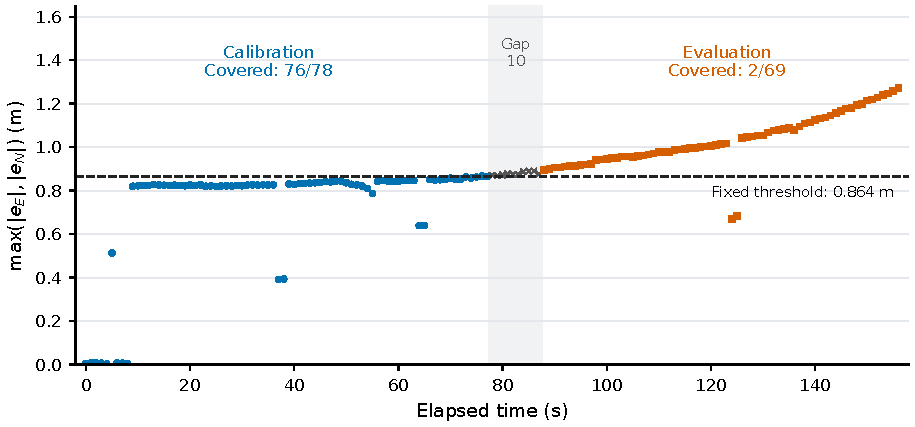
\includegraphics[width=\linewidth]{../figures/receiver_diagnostic.pdf}
\caption{Horizontal residual diagnostic for one stationary receiver. All 157 matched epochs are plotted, with a dashed line showing the 0.863506 m square half-width obtained from the calibration segment. Serial dependence and combined processing prevent interpreting this as online coverage performance.}\label{fig:receiver}
\end{figure}

\bibliography{references}
\end{document}
